% !TeX spellcheck = en_GB
%%%%%%%%%%%%%%%%%%%%%%%%%%%%%%%%%%%%%%%%%%
%                                        %
%    Engineer thesis LaTeX template      %
%  compliant with the SZJK regulations   %
%                                        %
%%%%%%%%%%%%%%%%%%%%%%%%%%%%%%%%%%%%%%%%%%
%                                        %
%  (c) Krzysztof Simiński, 2018-2023     %
%                                        %
%%%%%%%%%%%%%%%%%%%%%%%%%%%%%%%%%%%%%%%%%%
%                                        %
% The latest version of the templates is %
% available at                           %
% github.com/ksiminski/polsl-aei-theses  %
%                                        %
%%%%%%%%%%%%%%%%%%%%%%%%%%%%%%%%%%%%%%%%%%
%
%
% This LaTeX project formats the final thesis
% with compliance to the SZJK regulations.
% Please to not change formatting (fonts, margins,
% bolds, italics, etc).
%
% You can compile the project in several ways.
%
% 1. pdfLaTeX compilation
%
% pdflatex main
% bibtex   main
% pdflatex main
% pdflatex main
%
%
% 2. XeLaTeX compilation
%
% Compilation with the XeLaTeX engine inserts Calibri font
% in the title page. Of course the font has to be installed.
%
% xelatex main
% bibtex  main
% xelatex main
% xelatex main
%
%
%%%%%%%%%%%%%%%%%%%%%%%%%%%%%%%%%%%%%%%%%%%%%%%%%%%%%%%%%%%%%%
% If you have any questions, remarks, just send me an email: %
%            krzysztof.siminski(at)polsl.pl               %
%%%%%%%%%%%%%%%%%%%%%%%%%%%%%%%%%%%%%%%%%%%%%%%%%%%%%%%%%%%%%%

% We would like to improve the LaTeX templates
% of final theses. By answering the questions
% in the survey whose address your can find below
% you help us to do so. The survey is completely
% anonimous. Thank you!
%
% https://docs.google.com/forms/d/e/1FAIpQLScyllVxNKzKFHfILDfdbwC-jvT8YL0RSTFs-s27UGw9CKn-fQ/viewform?usp=sf_link
%
%%%%%%%%%%%%%%%%%%%%%%%%%%%%%%%%%%%%%%%%%%%%%%%%%%%%%%%%%%%%%%%%%%%%%%%%%

%%%%%%%%%%%%%%%%%%%%%%%%%%%%%%%%%%%%%%%%%%%%%%%
%                                             %
% CUSTOMISATION OF THE THESIS                 %
%                                             %
%%%%%%%%%%%%%%%%%%%%%%%%%%%%%%%%%%%%%%%%%%%%%%%

% Please customise your thesis with the macros below.

\newcommand{\Firstnames}{Krzysztof Marek}
\newcommand{\Surname}{Dziembała}
\newcommand{\Supervisor}{dr inż. Dominik Samociuk}
\newcommand{\Title}{Interactive security training platform based on CTF concept}
\newcommand{\TitleAlt}{Interaktywna platforma do nauki bezpieczeństwa wykorzystująca zadania typu CTF}
\newcommand{\Program}{Control, Electronic, and Information Engineering}
\newcommand{\Specialisation}{Informatics}
\newcommand{\Id}{293671}
\newcommand{\Departament}{OF COMPUTER NETWORKS AND SYSTEMS}


% If you have a consultant for your thesis, put their name below ...
% \newcommand{\Consultant}{$\langle$title first name surname$\rangle$}  %  (remove $\langle$ and $\rangle)
% ... else leave the braces empty:
\newcommand{\Consultant}{} % no consultant

% end of thesis customisation
%%%%%%%%%%%%%%%%%%%%%%%%%%%%%%%%%%%%%%%%%%

%%%%%%%%%%%%%%%%%%%%%%%%%%%%%%%%%%%%%%%%%%%%%%%
%                                             %
% END OF CUSTOMISATION                        %
%                                             %
%%%%%%%%%%%%%%%%%%%%%%%%%%%%%%%%%%%%%%%%%%%%%%%

%%%%%%%%%%%%%%%%%%%%%%%%%%%%%%%%%%%%%%%%


%%%%%%%%%%%%%%%%%%%%%%%%%%%%%%%%%%%%%%%%%%%%%%%
%                                             %
%   PLEASE DO NOT MODIFY THE SETTINGS BELOW!  %
%                                             %
%%%%%%%%%%%%%%%%%%%%%%%%%%%%%%%%%%%%%%%%%%%%%%%



\documentclass[a4paper,twoside,12pt]{book}
\usepackage[utf8]{inputenc}
\usepackage[T1]{fontenc}
\usepackage{amsmath,amsfonts,amssymb,amsthm}
\usepackage[polish,british]{babel}
\usepackage{indentfirst}



\usepackage{ifxetex}

\ifxetex
	\usepackage{fontspec}
	\defaultfontfeatures{Mapping=tex—text} % to support TeX conventions like ``——-''
	\usepackage{xunicode} % Unicode support for LaTeX character names (accents, European chars, etc)
	\usepackage{xltxtra} % Extra customizations for XeLaTeX
\else
	\usepackage{lmodern}
\fi



\usepackage[margin=2.5cm]{geometry}
\usepackage{graphicx}
\usepackage{hyperref}
\usepackage{booktabs}
\usepackage{tikz}
\usepackage{pgfplots}
\usepackage{mathtools}
\usepackage{geometry}
\usepackage{subcaption}   % subfigures
\usepackage[page]{appendix} % toc,




\usepackage{csquotes}
% I know that students are NOT ALLOWED to change it and the behaviour was expected,
% but my supervisor wants bibliography sorted in order of first appearance.
\usepackage[natbib=true,backend=bibtex,maxbibnames=99,sorting=none]{biblatex}  % compilation of bibliography with BibTeX
%\usepackage[natbib=true,backend=biber,maxbibnames=99,sorting=none]{biblatex}  % compilation of bibliography with Biber
\bibliography{biblio/biblio}

\usepackage{ifmtarg}   % empty commands

\usepackage{setspace}
\onehalfspacing


\frenchspacing



%%%% TODO LIST GENERATOR %%%%%%%%%

\usepackage{color}
\definecolor{brickred}      {cmyk}{0   , 0.89, 0.94, 0.28}

\makeatletter \newcommand \kslistofremarks{\section*{Remarks} \@starttoc{rks}}
  \newcommand\l@uwagas[2]
    {\par\noindent \textbf{#2:} %\parbox{10cm}
{#1}\par} \makeatother


\newcommand{\ksremark}[1]{%
{%\marginpar{\textdbend}
{\color{brickred}{[#1]}}}%
\addcontentsline{rks}{uwagas}{\protect{#1}}%
}










%%%%%%%%%%%%%% END OF TODO LIST GENERATOR %%%%%%%%%%%

%%%%%%%%%%%% FANCY HEADERS %%%%%%%%%%%%%%%
% no capitalisation of headers
\usepackage{fancyhdr}
\pagestyle{fancy}
\fancyhf{}
\fancyhead[LO]{\nouppercase{\it\rightmark}}
\fancyhead[RE]{\nouppercase{\it\leftmark}}
\fancyhead[LE,RO]{\it\thepage}


\fancypagestyle{onlyPageNumbers}{%
   \fancyhf{}
   \fancyhead[LE,RO]{\it\thepage}
}

\fancypagestyle{noNumbers}{%
   \fancyhf{}
   \fancyhead[LE,RO]{}
}


\fancypagestyle{PageNumbersChapterTitles}{%
   \fancyhf{}
   \fancyhead[LO]{\nouppercase{\Firstnames\ \Surname}}
   \fancyhead[RE]{\nouppercase{\leftmark}}
   \fancyfoot[CE, CO]{\thepage}
}




%%%%%%%%%%%%%%%%%%%%%%%%%%%







\newcounter{pagesWithoutNumbers}

%%%%%%%%%%%%%%%%%%%%%%%%%%%
\usepackage{xstring}
\usepackage{ifthen}
\newcommand{\printOpiekun}[1]{%

    \StrLen{\Consultant}[\mystringlen]
    \ifthenelse{\mystringlen > 0}%
    {%
       {\large{\bfseries CONSULTANT}\par}

       {\large{\bfseries \Consultant}\par}
    }%
    {}
}
%
%%%%%%%%%%%%%%%%%%%%%%%%%%%%%%%%%%%%%%%%%%%%%%

% Please do not modify the lines below!
\author{\Firstnames\ \Surname}
\newcommand{\Author}{\Firstnames\ \MakeUppercase{\Surname}}
\newcommand{\Type}{FINAL PROJECT}
\newcommand{\Faculty}{Faculty of Automatic Control, Electronics and Computer Science}
\newcommand{\Polsl}{Silesian University of Technology}
\newcommand{\Logo}{graf/politechnika_sl_logo_bw_pion_en.pdf}
\newcommand{\LeftId}{Student identification number}
\newcommand{\LeftProgram}{Programme}
\newcommand{\LeftSpecialisation}{Specialisation}
\newcommand{\LeftSUPERVISOR}{SUPERVISOR}
\newcommand{\LeftDEPARTMENT}{DEPARTMENT}
%%%%%%%%%%%%%%%%%%%%%%%%%%%%%%%%%%%%%%%%%%%%%%

%%%%%%%%%%%%%%%%%%%%%%%%%%%%%%%%%%%%%%%%%%%%%%%
%                                             %
% END OF SETTINGS                             %
%                                             %
%%%%%%%%%%%%%%%%%%%%%%%%%%%%%%%%%%%%%%%%%%%%%%%

 % Do not modify!


%%%%%%%%%%%%%%%%%%%%%%%%%%%%%%%%%%%%%%%%%%%%%%%
%                                             %
% MY PACKAGES, SETTINGS ETC.                  %
%                                             %
%%%%%%%%%%%%%%%%%%%%%%%%%%%%%%%%%%%%%%%%%%%%%%%

% Put your packages, macros, setting here.



%%%%%%%%%%%%%%%%%%%%%%%%%%%%%%%%%%%%%%%%%%%%%%%%%%%%%%%%%%%%%%%%%%%%%
% listings
% packages: listings or minted
% % % % % % % % % % % % % % % % % % % % % % % % % % % % % % % % % % %

% package listings
% \usepackage{listings}
% \lstset{%
% morekeywords={string,exception,std,vector},% add the keyword you need
% language=C++,% C, Matlab, Python, SQL, TeX, XML, bash, ... – vide https://www.ctan.org/pkg/listings
% commentstyle=\textit,%
% identifierstyle=\textsf,%
% keywordstyle=\sffamily\bfseries, %\texttt, %
% %captionpos=b,%
% tabsize=3,%
% frame=lines,%
% numbers=left,%
% numberstyle=\tiny,%
% numbersep=5pt,%
% breaklines=true,%
% %morekeywords={descriptor_gaussian,descriptor,partition,fcm_possibilistic,dataset,my_exception,exception,std,vector},%
% escapeinside={@*}{*@},%
% }

% % % % % % % % % % % % % % % % % % % % % % % % % % % % % % % % % % %
% package minted
\usepackage{minted}

% minted 2.7 quotes command-line arguments, this allows us to escape the quotes
% and pass arguments directly to pygmentize, forcing it to use custom lexer.
% Quoting lexer argument: https://github.com/gpoore/minted/blob/9ac85a3a1ae09936d80daf46927f55c51449555b/source/minted.sty#L842
% Quoting macro: https://github.com/gpoore/minted/blob/9ac85a3a1ae09936d80daf46927f55c51449555b/source/minted.sty#L820-L824
\usepackage{ifplatform}
\makeatletter
\@ifpackagelater{minted}{2022/12/12}{
	\ifwindows
		\newenvironment{mintedlexer}[1]{\minted{#1" "-x}}{\endminted}
	\else
		\newenvironment{mintedlexer}[1]{\minted{#1' '-x}}{\endminted}
	\fi
}{
	\newenvironment{mintedlexer}[1]{\minted{#1 -x}}{\endminted}
}
\makeatother

% This package requires a special command line option in compilation
% pdflatex -shell-escape main.tex
% xelatex  -shell-escape main.tex

%%%%%%%%%%%%%%%%%%%%%%%%%%%%%%%%%%%%%%%%%%%%%%%%%%%%%%%%%%%%%%%%%%%%%

% PlantUML diagrams are rendered to svg, so svg is required to include them
% plantuml package works only with lualatex
% TikZ figures generated with -tlatex:nopreamble are not displayed correctly
\usepackage{svg}


%%%%%%%%%%%%%%%%%%%%%%%%%%%%%%%%%%%%%%%%%%%%%%%
%                                             %
% END OF MY PACKAGES, SETTINGS ETC.           %
%                                             %
%%%%%%%%%%%%%%%%%%%%%%%%%%%%%%%%%%%%%%%%%%%%%%%

 % Put your settings, packages, macros here.

%%%%%%%%%%%%%%%%%%%%%%%%%%%%%%%%%%%%%%%%


\begin{document}
%\kslistofremarks


%%%%%%%%%%%%%%%%%%%%%%%%%%%%%%%%%%%%%%%%%%%%%%%
%                                             %
%    PLEASE DO NOT MODIFY THE TITLE PAGE!     %
%                                             %
%%%%%%%%%%%%%%%%%%%%%%%%%%%%%%%%%%%%%%%%%%%%%%%


%%%%%%%%%%%%%%%%%%  TITLE PAGE %%%%%%%%%%%%%%%%%%%
\pagestyle{empty}
{
	\newgeometry{top=1.5cm,%
	             bottom=2.5cm,%
	             left=3cm,
	             right=2.5cm}

	\ifxetex
		\begingroup
		\setsansfont{Calibri}
	\else \ifluatex
			\begingroup
			\setsansfont{Calibri}
		\fi
	\fi
	\sffamily
	\begin{center}
	\includegraphics[width=50mm]{\Logo}


	{\Large\bfseries\Type\par}

	\vfill  \vfill

	{\large\Title\par}

	\vfill

	{\large\bfseries\Author\par}

	{\normalsize\bfseries \LeftId: \Id}

	\vfill

	{\large{\bfseries \LeftProgram:} \Program\par}

	{\large{\bfseries \LeftSpecialisation:} \Specialisation\par}

	\vfill  \vfill 	\vfill 	\vfill 	\vfill 	\vfill 	\vfill

	{\large{\bfseries \LeftSUPERVISOR}\par}

	{\large{\bfseries \Supervisor}\par}

	{\large{\bfseries \LeftDEPARTMENT\ \Departament} \par}

	{\large{\bfseries \Faculty}\par}

	\vfill  \vfill


    \printOpiekun{\Consultant}

	\vfill  \vfill

    {\large\bfseries  Gliwice \the\year}

	\end{center}
	\ifxetex
		\endgroup
	\else \ifluatex
			\endgroup
		\fi
	\fi
	\restoregeometry
}

  % Please to not modify the titlepage.tex file!

\cleardoublepage

\rmfamily\normalfont
\pagestyle{empty}


%%% Let's start the thesis %%%%

\subsubsection*{Thesis title} \Title

\subsubsection*{Abstract}
The popularity of the internet and its broad usage in the contemporary world introduces new problems in the form of vulnerabilities. One of the best ways to prevent them is good and practical cybersecurity education of developers responsible for the said web services. The thesis aims to design and create an easy-to-use platform suitable for education about web security using capture the flag challenges. The project combines this popular type of tasks with multiple-choice quizzes and allows rich descriptions of vulnerability types. The solution uses Docker and nginx proxy for easy automated challenge management.

\subsubsection*{Keywords}
educational platform, cybersecurity training, CTF, web security, Docker

\subsubsection*{Tytuł pracy}
\begin{otherlanguage}{polish}
\TitleAlt
\end{otherlanguage}

\subsubsection*{Streszczenie}
\begin{otherlanguage}{polish}
Popularność internetu i jego powszechne użytkowanie we współczesnym świecie przyczynia się do powstawania nowego problemu w postaci luk bezpieczeństwa. Jednym z najlepszych sposobów zapobiegania temu problemowi jest dobra i praktyczna edukacja deweloperów aplikacji webowych z zakresu cyberbezpieczeństwa. Celem pracy jest zaprojektowanie i stworzenie łatwej w użytkowaniu platformy przeznaczonej do edukacji o bezpieczeństwie aplikacji internetowych wykorzystującej wyzwania capture the flag. Projekt łączy ten popularny rodzaj zadań z pytaniami wielokrotnego wyboru i pozwala na bogate opisy rodzajów podatności. Rozwiązanie wykorzystuje Dockera i proxy nginx do łatwego i zautomatyzowanego zarządzania wyzwaniami.
\end{otherlanguage}
\subsubsection*{Słowa kluczowe}
\begin{otherlanguage}{polish}
platforma edukacyjna, nauczanie cyberbezpieczeństwa, CTF, bezpieczeństwo aplikacji internetowych, Docker
\end{otherlanguage}

 % editorials


%%%%%%%%%%%%%%%%%% Table of contents %%%%%%%%%%%%%%%%%%%%%%
%\pagenumbering{Roman}
\thispagestyle{empty}
\tableofcontents
\thispagestyle{empty}

%%%%%%%%%%%%%%%%%%%%%%%%%%%%%%%%%%%%%%%%%%%%%%%%%%%%%
\setcounter{pagesWithoutNumbers}{\value{page}}
\mainmatter
\pagestyle{empty}

\cleardoublepage

\pagestyle{PageNumbersChapterTitles}

%%%%%%%%%%%%%% body of the thesis %%%%%%%%%%%%%%%%%

\chapter{Introduction}

\begin{itemize}
\item introduction into the problem domain
\item settling of the problem in the domain
\item objective of the thesis
\item scope of the thesis
\item short description of chapters
\item clear description of contribution of the thesis's author – in case of more authors table with enumeration of contribution of authors
\end{itemize}


\chapter{Problem analysis}

Traditional capture the flag game requires the player to take a flag or a similar object from the opponent's base and bring it back to their own. Similarly, in cybersecurity CTF the objective is to obtain a flag from the \textit{opponent}. There are two formats of CTFs - attack-defence and jeopardy. In the first type competing teams have to both attack other teams and protect their own system. The latter requires participants to \textit{steal} the flags from organiser-prepared challenges. The tools developed for this thesis are supposed to help programmers understand security issues, therefore only jeopardy-style tasks are considered.

\section{Literature research}

Using CTF-style challenges for cybersecurity education is not a new idea. Gamification is helpful for increasing user engagement and works in cybersecurity too \cite{bib:exploring-game-design}. An analysis of PicoCTF 2013 competition by Chapman et al. \cite{bib:picoCTF} shows that properly prepared CTFs are suitable even for high school students with no security experience. According to the survey answers, the teachers observed that the students put more effort into the CTF than usually during lessons.

\subsection{CTF as university laboratories}

CTF challenges have already been used during cybersecurity laboratories on some universities. The topic has been approached in various ways by the instructors.

Karagiannis and Magkos \cite{bib:Karagiannis2021} use CTFd for managing the challenges. Challenges were divided into subsequent steps to guide the participants through the process and present the knowledge better. \href{https://vulnhub.com/}{VulnHub} VMs were used as the challenges and most of them were running locally on students' computers.

In \cite{bib:teaching-ctf-PL} Ksiezopolski et al. present their web application security course based on CTF. Students connect to the infrastructure using individual VPN configurations. A challenge must be started by a student using a web portal to make it available on the VPN network. This solution allows \textit{cheap} scaling by starting challenges as required.

\subsection{Technical details of CTF organization}

CERT Polska describes their approach to hosting CTF competitions in \cite{bib:hack.cert.pl}. Their solution for hosting \textit{web} and \textit{pwn} challenges is based on Docker Compose. This decision allows them to use different environments for each challenge, which should behave identically on different devices, therefore eliminating compatibility problems. Routing network traffic to appropriate containers is achieved by using server blocks with \mintinline{nginx}|server_name| and \mintinline{nginx}|proxy_pass| directives in nginx configuration files.

Authors detail also their remarks regarding task design. The article suggests using NsJail to prevent accidental or purposeful denial of service (DOS) on high-risk challenges such as those leading to RCE. Another helpful idea is using \href{https://github.com/Supervisor/supervisor}{supervisord} for managing multiple processes inside a single container.

\section{Existing solutions}
\label{sec:existing-solutions}

There are many open-source platforms developed for hosting CTF competitions and some of them were created with education in mind. This section shortly describes some of the most popular solutions which could be used to introduce CTF challenges in the context of education. However, the presented projects frequently solve only a part of the problem - either providing the user interface or the infrastructure for hosting challenges.

\subsection{CyTrONE}

\href{https://github.com/crond-jaist/cytrone}{CyTrONE} \cite{bib:cytrone} is a cybersecurity training framework developed at the Japan Advanced Institute of Science and Technology. The system operates on virtual machines hosting the vulnerable applications which are created based on YAML configuration files. The VMs are cloned for each student requesting a \textit{cyber range}. Guest VMs may include a desktop with tools required for exploitation, so that users can simply connect to the VM and use the tools available there. Besides \textit{cyber ranges}, the system supports also text and multiple-choice quizzes. Administrators (called \textit{training coordinators}) manage the database of \textit{cyber ranges} and quizzes using a web UI or iOS application. Students have access to the training through the Moodle learning management system which CyTrONE closely integrates with.

\subsection{kCTF}

\href{https://github.com/google/kctf}{kCTF} is a Kubernetes-based infrastructure for hosting CTFs developed by Google. Thanks to the use of Kubernetes the challenges should scale automatically as required. The templates available for kCTF include healthcheck containers and use NsJail for sandboxing the incoming connections and securing challenges with remote code execution. kCTF provides only the infrastructure, so the user interface must be deployed separately.

\subsection{CTFd}
\label{ssec:CTFd}

\href{https://github.com/CTFd/CTFd}{CTFd} is a highly configurable CTF framework. Challenges can be configured in such a way that they must be solved in appropriate order. It supports plugins which extend the functionality. One of the advantages appreciated by the users of CTFd is its clear UI which is intuitive even for beginners \cite{bib:CTF-analysis, bib:bangladesh-CTFd}. Unfortunately, the official multiple choice challenge plugin is available only in paid versions. The targets for web challenges can only be linked to and must be hosted separately.

\subsection{FBCTF}
\label{ssec:FBCTF}

\href{https://github.com/facebookarchive/fbctf}{Facebook CTF (FBCTF)} is a \textbf{deprecated} platform for hosting CTF competitions. Since it targets mostly competitions it has a highly-configurable scoring system. Besides jeopardy-style challenges it supports also quizzes (with text answers) and \textit{King of the hill} games in which teams compete for control over a target system. The \textit{flag levels}, which are the jeopardy tasks, have a file or a link to the target attached, but how the target system is maintained is left up to the administrator. According to Karagiannis et al. \cite{bib:CTF-analysis}, FBCTF is best suited for organizing CTF competitions as events.

\subsection{Mellivora}

\href{https://github.com/Nakiami/mellivora}{Mellivora} is a very lightweight and simple CTF engine. It allows \textit{challenge chains} where a task becomes available only after a different specific challenge has been solved. Challenges have a BBCode description and can contain files, but if a web service is required it must be hosted separately and linked in the description. Answers must be in a text form and can be marked automatically or manually by the administrators.

\subsection{Root the Box}

\href{https://github.com/moloch--/RootTheBox}{Root the box} is a CTF scoring engine with many configurable features. It supports multiple flag types including text (static and regular expressions), datetime, multiple choice and file, which may be really useful when used for educational purposes. Support for the \href{https://github.com/juice-shop/juice-shop-ctf}{Juice Shop CTF CLI} makes it easy to add challenges from that CTF, however this feature does not differentiate it from \hyperref[ssec:CTFd]{CTFd} and \hyperref[ssec:FBCTF]{FBCTF}, which are also supported. However, Karagiannis et al. \cite{bib:CTF-analysis} claims that Root the Box is too complex for beginners, therefore not a good solution for education.


\chapter{Requirements and tools}
\label{chap:req-and-tools}

The project development consisted of multiple stages. One of the most important parts was specifying requirements, which then dictated tool selection and the design process.

\section{Functional requirements}

Functional requirements list functionality available in the system. Each of the requirements contains a description detailing the desired behaviour.

\begin{enumerate}
	\item \textbf{Account creation}: Users must be able to register an account in the system.
	This operation requires username and password submission from an HTML form in a POST request.
	Registration is allowed only using a unique username. If there already exists an account in the system with the same username, the action must be refused.
	As a result of a successful registration, a document with the username, cryptographic hash of the user's password and a default role \texttt{"user"} is inserted into a collection storing user accounts. After the registration succeeds, the user is redirected to the login page.

	\item \textbf{Signing in}: Users must be able to log into their accounts.
	Username and password must be sent in a POST request as HTML form data. The operation must fail if there is no account in the database with the provided username or if the password hash does not match the one stored in the database.
	If there has been no failure, a session is created and the user is redirected to the home page.

	\item \textbf{Logging out}: Users must be able to log out of their accounts.
	It is expected that the user is signed in when they log out. This operation destroys the session (if any) and redirects to the home page.

	\item \textbf{Changing password}: Users must be able to change their account password.
	New password must be sent in a POST request as HTML form data. User must be logged-in in order to change the password.
	As a result of this operation, user's password hash in the database is updated.

	\item \textbf{Listing categories}: Users must be able to see a list of categories that exist in the system. The list of categories must link to category pages.

	\item \textbf{Displaying category}: Users must be able to see category details on a category page. The details should include category name, description and a list of related tasks.

	\item \textbf{Displaying task}: Users must be able to display task details on task pages. The details should include task name, description, challenge URL, hints (if any), and if the user is logged in, a flag submission form. If the task has been solved by the user, instead of the flag submission form, a question is displayed.

	\item \textbf{Solving challenge}: Users must be able to submit a form with a flag from the task page. This action is allowed only for signed-in users. The submitted flag must be verified with the one stored in the database for the given challenge. If the flags match, a success message should be shown to the user and the date of solving the challenge by user ought to be saved to the database. Otherwise, a message informing the user about an incorrect flag should be presented.

	\item \textbf{Answering quiz}: Users who have solved the main challenge from a task, should be able to see a question on the task page and be able to answer it. Only signed-in users can submit answers. Checkboxes whose status indicates whether the user thinks that they are correct must be presented along answers from the database. After the answers are submitted, the quiz should be disabled without a button to submit, checkboxes disabled and reflecting the user's answer and an indication which answers were correct.

	\item \textbf{Administrator panel}: Users with the \texttt{"admin"} role (administrators) should have access to a separate administration panel. The panel should expose additional functionality related to the system management.

	\item \textbf{Listing users}: Users with access to the administrator panel should be able to get a list of user accounts in the system. Each entry must contain information about username and user role. The list should be paginated, as there may exist many accounts.

	\item \textbf{Changing user permissions}: Administrators should be able to grant the \texttt{"admin"} role to other users, as well as change it back to \texttt{"user"}.

	\item \textbf{Deleting user}: Administrators should be able to remove user accounts from the database. It must not be possible for the administrator to remove their own user account this way.

	\item \textbf{Creating category}: Administrators must be able to create new categories. The categories must have a name and description. The description must support Markdown input.

	\item \textbf{Editing category}: Administrators must be able to edit the name and description of existing categories.

	\item \textbf{Creating task}: Administrators must be able to add new tasks to the system. For each task it must be possible to set the name, description (in Markdown), hints, challenge details, question, answers to the question. Each answer must be marked as correct or incorrect.\\
	Challenge details must include:
	\begin{itemize}
		\item a Docker image to pull and start,
		\item a subdomain used for serving the challenge,
		\item a flag that the users will try to find,
		\item an interval specifying how frequently the challenge container should be regenerated.
	\end{itemize}

	\item \textbf{Starting challenges}: The system must be able to pull challenge images, create and start containers and direct connections to specified subdomains into appropriate containers. This must be done automatically during system startup and for each new challenge added when creating new tasks.
\end{enumerate}

Functional requirements are related to actions that the system offers to actors using it. These actions are presented by the use case diagram in Fig. \ref{fig:use-case-diag}. There are two actors, with different sets of allowed interactions. The actor \textit{User} represents anyone with access to the system. Administrators are users with a special account role \texttt{"admin"}, which allows them to perform operations related to management of the system.

\begin{figure}
	\centering
	\includesvg[inkscapelatex=false,scale=0.9]{uml/render/usecase.svg}
	\caption{Use case diagram.}
	\label{fig:use-case-diag}
\end{figure}

\section{Non-functional requirements}

Non-functional requirements listed below describe project evaluation criteria not related to specific system behaviours.

\begin{enumerate}
	\item \textbf{Responsiveness}: UI should properly scale across different display sizes. It must be mobile-friendly.

	\item \textbf{Accessibility}: There should be no errors in the Accessibility section of a \href{https://webhint.io/}{webhint} scan.

	\item \textbf{Visual consistency}: A single set of styling rules, such as colours, fonts and icons should be used across the whole user interface.

	\item \textbf{Page load performance}: The system should have a score of over 90 in \href{https://pagespeed.web.dev}{PageSpeed Insights} report for mobile.

	\item \textbf{Compatibility}: User interface should work in the latest (as of January 2023) versions of Firefox, Firefox ESR, Chrome and Safari browsers for desktops and mobile devices. Basic system functionality, except for the administrator panel, should be available in browsers with JavaScript disabled.
\end{enumerate}

\section{Tools}

The implementation of the project significantly benefited from publicly available tools. Used tools are divided into two classes, depending on the way they were used.

\subsection{Core tools}

The system is built on tools, which are regarded to as \textit{core tools}. These are required for operation and are a part of the system architecture.

\subsubsection{Node.js + Express + EJS}

Node.js is a JavaScript runtime based on V8 engine. There is an enormous ecosystem built around Node.js with over 1.3 million packages available in the npm registry \cite{bib:npm-packages}. The server code runs on Node.js and uses the Express framework for request routing and middleware management. Express is a popular web framework with many features and compatible middleware packages. One of Express' features is template rendering support. The project uses EJS templates which allow creating HTML templates using embedded JavaScript logic.

\subsubsection{MongoDB}

MongoDB is a NoSQL document-oriented database capable of storing BSON documents. Because BSON stands for Binary JSON, which in turn is JavaScript Object Notation, it integrates nicely with JavaScript. The MongoDB Node.js driver also supports TypeScript, which helps with suggestions and type checking.\\
During development MongoDB Compass, MongoDB Visual Studio Code extension and mongosh were used. These tools allow database management and, except for mongosh, provide helpful user interfaces.

\subsubsection{Docker}

Docker is a platform for managing containerized software. Challenges are running as Docker containers and managed using Docker Engine API. For debugging, development and management, standalone Docker tools such as Docker CLI and Docker Desktop can be used.

\subsubsection{nginx}

To manage multiple domains and subdomain on a single system with one external network interface nginx was used as a proxy. nginx offers multiple functionalities besides proxying. It is also used to serve static files, redirect to HTTPS protocol and terminate TLS connections.

\subsubsection{Bootstrap}

Bootstrap is a frontend toolkit, which is helpful for designing user interfaces. It provides CSS classes and JavaScript utilities to help with styling and providing interactivity in HTML without the need to write own style sheets and JS scripts.

\subsection{Development tools}

The following tools are not required for the systems to be fully operational. These were used to aid development.

\subsubsection{Visual Studio Code}

Visual Studio Code is a multi-platform code editor that was heavily used for writing the software. It was chosen for multiple reasons, most important of which was familiarity and experience with the tool. This editor supports many languages, especially for JavaScript and related web technologies. Particularly notable is built-in TypeScript support, which can be used with JSDoc comments to improve IntelliSense suggestions. A huge advantage of Visual Studio Code is a broad selection of available extensions.

\subsubsection{Git}

The project is stored in a Git repository to track changes in the code. The repository is synchronized with GitHub to share it between devices.

\subsubsection{ESLint}

ESLint is a JavaScript linter, which can be used to detect problems and potential issues in code. It was used with a Visual Studio extension, which automatically analysed open files and provided in-editor warnings and suggestions.

\subsubsection{Prettier}

Prettier is a popular code formatting tool. It was used to maintain a consistent style in JavaScript files. Thanks to Visual Studio Code plug-in, the tool could be used as a default formatter in the editor. A plug-in for ESLint allowed marking improperly formatted code as lint error.

\section{Methodology of design and implementation}

The development process was split into two parts. Before the implementation started, the system had to be designed.

\subsection{Design}

The first step in designing the project was defining initial requirements.
This resulted in the first (and only) UI concept drawing, which is presented in Fig. \ref{fig:init-ui-sketch}. It was meant to help with defining the exact functionality and the structure of documents in the database. Based on that the structure presented in Fig. \ref{fig:init-db-struct} was created.

After those first ideas were noted, the process of defining the architecture began. The choice of Node.js and Express as a base for the server was easy, as the author had significant experience with those tools. Similarly, MongoDB was selected as a database server, because of earlier experience and because it can store arrays and objects. To improve experience on low-end devices and enable basic functionality on browsers without JavaScript, server-side rendering was chosen instead of a JavaScript user interface library such as React or Vue. For a template rendering engine two solutions were considered - Handlebars and EJS. Ultimately, EJS was chosen due to its richer capabilities.

The last problem to solve during the design phase was coming up with an idea to direct different subdomains to appropriate challenge containers. The simplest solution was using a wildcard DNS record and setting up virtual servers in the proxy (Fig. \ref{fig:subdomain-idea}). Creation of subdomains could be achieved by creating additional configuration files, which could be automatically picked up by the proxy on reload.

\begin{figure}
	\centering
	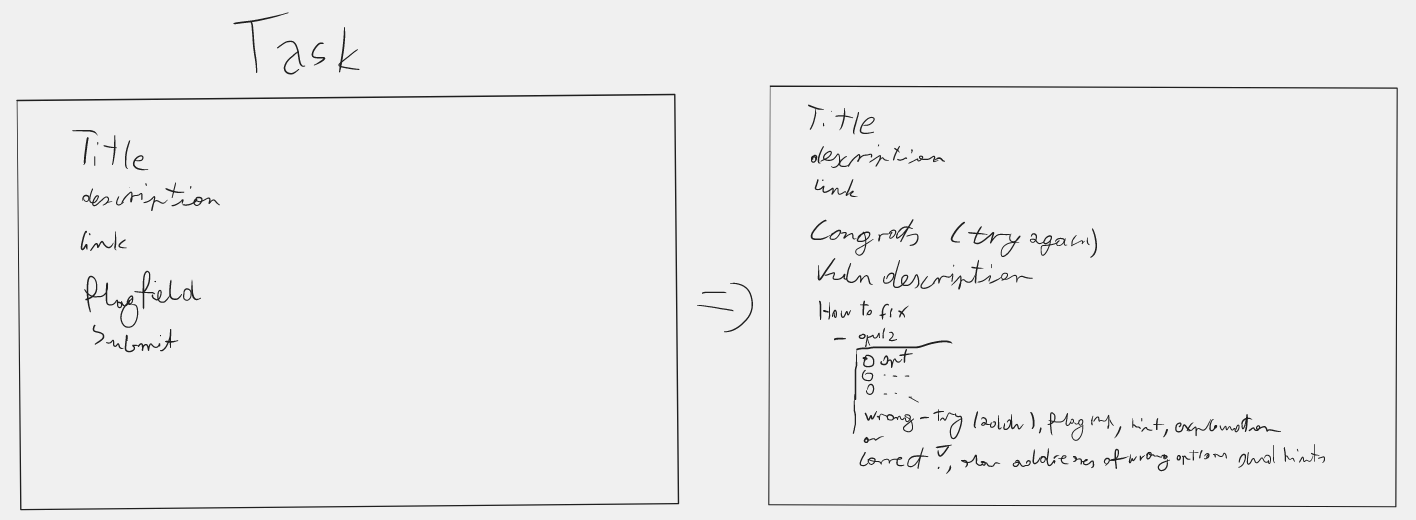
\includegraphics[width=\textwidth]{img/init-ui-sketch.png}
	\caption{Initial task page UI sketch before and after solving the challenge.}
	\label{fig:init-ui-sketch}
\end{figure}

\begin{figure}
	\centering
	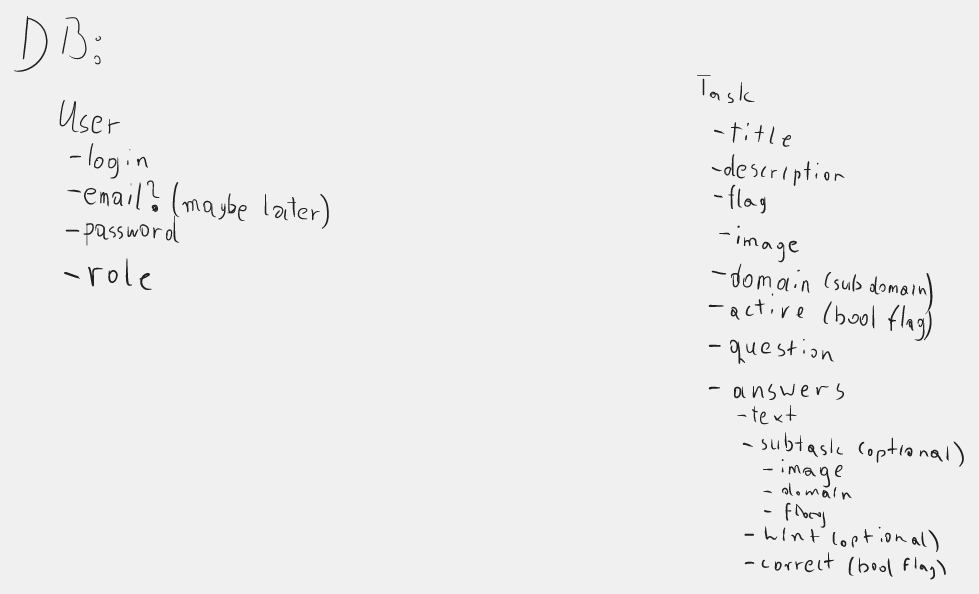
\includegraphics[width=\textwidth]{img/init-db-struct.png}
	\caption{Initial design of documents representing users and tasks.}
	\label{fig:init-db-struct}
\end{figure}

\begin{figure}
	\centering
	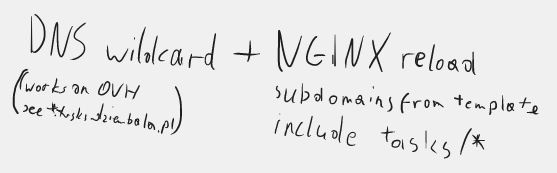
\includegraphics[width=\textwidth]{img/subdomain-idea.png}
	\caption{Subdomain management design idea.}
	\label{fig:subdomain-idea}
\end{figure}

\subsection{Implementation}

The implementation started with setting up a Node.js project with some required dependencies and a basic \textit{Hello world} Express server. Additional tools such as ESLint were also set up at the beginning, so that they could be used during the development.

The next step was preparing database connection and setting up code for session support. Once the server could handle sessions, related utilities such as message flashing were prepared. Sessions were required to implement authentication, which was done in the next step. The first part of implementing authentication was enabling user account creation, so that it would be possible to test each element as it was developed. With the code responsible for registration ready, logging in could be worked on. In both cases the server logic was prepared first with the UI following right after to test the whole component.

After the authentication was done and there were some simple pages ready, work on styling the interface could begin. This stage of the development was realized at that moment, because there were already pages which could be tested with the styles and could serve as a base for later content.

Before more public pages could be created, an administration panel had to be made in order to insert data for testing. Unlike all other components, this panel required a lot of interactivity and relied on client-side scripting. To facilitate this requirement, the server code exposes REST-like API, which is consumed by scripts running in the browser. The administrator panel started with user management, continued to category management and finished with task creation.\\
Since some inputs supported Markdown, a Markdown parser was integrated on both the server and in browser. To allow for syntax highlighting in code blocks, \href{https://highlightjs.org}{highlight.js} was added to the Markdown parser. Syntax highlighting required additional styles, which were available separately in light and dark modes and would not integrate well with Bootstrap's theming. To avoid this problem, a variable-based style sheet with colours from Panda Syntax Light and Dark themes was created with CSS variables set depending on the theme used in Bootstrap.\\
With the last part of the administration panel, task creation, a system for managing challenge containers had to be prepared. During the implementation of this functionality, the initial database schema shown in Fig \ref{fig:init-db-struct} was recognized as suboptimal and had to be changed.

Finally, user-facing category and task pages were prepared. These were template-based and in case of the task page relatively complicated, so the user interface and server code could be implemented in parallel. As a finishing touch a simple home page was added.


% TODO
\chapter{External specification}

The external specification contains information important for the users and administrators of the system. This chapter describes necessary requirements for system usage, presents relevant instructions and other useful details.

\section{Hardware and software requirements}

Depending on whether one wants to use the user interface via a web browser or host the server themselves there are different requirements for each part.

\subsection{Browser}

The user interface requires a modern browser with JavaScript enabled. It is possible to use the system without JS, but theme switching and dropdowns in the navigation bar will not work.

On desktop the latest stable versions of the following browsers are supported:

\begin{itemize}
    \item Google Chrome,
    \item Microsoft Edge,
    \item Firefox and Firefox ESR,
    \item Opera,
    \item Safari (macOS only).
\end{itemize}

On Android and iOS support is restricted to the latest stable versions of:

\begin{itemize}
    \item Google Chrome,
    \item Firefox,
    \item Safari (iOS only),
    \item Android Browser and WebView (Android only).
\end{itemize}

Different and older browsers may work, but compatibility is not guaranteed.

\subsection{Server software}
\label{chap:server-soft}

The server software requires the following external software to be installed:

\begin{itemize}
    \item Node.js 18.x or newer (not as a \href{https://snapcraft.io/node}{snap}),
    \item MongoDB 6.0,
    \item Docker Engine 20.10,
    \item nginx 1.23.2 or newer.
\end{itemize}

Supported operating systems:

% https://github.com/ranisalt/node-argon2/tree/v0.30.3#prebuilt-binaries
\begin{itemize}
    \item Ubuntu 20.04 or newer (x86-64, arm64),
    \item macOS 11 (x86-64), 12 or newer (x86-64, arm64),
    \item Windows 10 1809 or newer (x86-64),
    \item Windows Server 2019 or newer (x86-64).
\end{itemize}

It may be possible to run the server on other operating systems and architectures as long as the required software can be installed. These unsupported systems, however, will probably require \href{https://github.com/ranisalt/node-argon2/tree/v0.30.3#before-installing}{additional installation steps} related to \texttt{argon2} package setup.

\textbf{Warning:} Challenge Docker images must be compatible with the server architecture. Images presented in this project support only x86-64.

\section{Server installation}

The process of server software installation and configuration can be summarized in the following steps:

\begin{enumerate}
    \item Install the required software as described in section \ref{chap:server-soft}.
    \item Obtain the code from GitHub:\\
    \mintinline{bash}|git clone https://github.com/krzysdz/inz.git|
    \item Navigate to the downloaded project directory:\\
    \mintinline{bash}|cd inz|
    \item Install required npm packages:\\
    \mintinline{bash}|npm install --omit=dev|
    \item Configure MongoDB as a replica set (\href{https://www.mongodb.com/docs/manual/tutorial/deploy-replica-set/}{tutorial}).
    \item Configure the DNS to point the main domain and the challenges domain to the server. Example DNS configuration:
    \begin{mintedlexer}{DNSLexer.py:DNSLexer}
main-ui.com.        60  IN A        127.0.0.1
*.challenges.com.   60  IN CNAME    main-ui.com.
    \end{mintedlexer}
    \item Obtain TLS certificate for the main domain and the challenges domain. One certificate should cover both domains (the second one with wildcard).\\
    The key and certificate files should be placed in \texttt{nginx/certs} and named according to instructions from the \texttt{README} file in that directory.
    \item Adjust values in the \texttt{config.js} file.
    \item Start nginx with prefix set to \texttt{./nginx} and configuration \texttt{nginx/conf/nginx.conf}:\\
    \mintinline{bash}|nginx -p ./nginx -c ./nginx/conf/nginx.conf|
    \item Set \texttt{NODE\_ENV} to production:

    Bash/dash/zsh/csh:\\
    \mintinline{bash}|export NODE_ENV="production"|

    Powershell:\\%TC:ignore
    \mintinline{pwsh}|$env:NODE_ENV="production"|%TC:endignore
    \item Start the server:\\
    \mintinline{bash}|node index.js|

    \item \textit{Optional.} Configure services to automatically start the software. Example configuration for systemd based operating systems:
    \begin{enumerate}
        \item Modify the default mongod.conf file to specify replica set name as shown on Fig. \ref{fig:example-mongod} and enable the \href{https://github.com/mongodb/mongo/blob/e4fff3e1fe7b31b25cedde7b05205325b47b4a7d/debian/mongod.service}{mongod service}:\\
        \mintinline{bash}|systemctl enable mongod|
        \item Create a unit file for the proxy. An example is presented on Fig. \ref{fig:example-nginx-service}.
        \item Create a unit file for the main server. An example is presented on Fig. \ref{fig:example-server-service}.
        \item Enable and start the services:
        \begin{minted}{bash}
# Reload systemd configuration to pick up the new services
systemctl daemon-reload
# Enable the services to run at boot
systemctl enable inz-nginx
systemctl enable inz
# Start the server and proxy (required by inz.service)
systemctl start inz
        \end{minted}
    \end{enumerate}
\end{enumerate}

\section{Initial configuration}

If setting up the server with a fresh database, an administrator account must be created. To do this, one has to:

\begin{itemize}
    \item Create a user account (\texttt{/auth/register}).
    \item Set the \texttt{role} field of the user document to string \texttt{admin}. A Node.js script which does that is presented on Fig. \ref{fig:make-admin-script}.
    \item Log in into the account again.
\end{itemize}

\section{Types of users}
\label{chap:types-of-users}

There are three types of users considered in the system:
\begin{itemize}
    \item anonymous/not signed in,
    \item regular users - account with role \texttt{"user"},
    \item administrators - account with role \texttt{"admin"}.
\end{itemize}

Anonymous users can freely browse the application, but have a limited functionality on the task page.\\
Regular users gain access to profile page and unlock challenge and quiz submissions.\\
Administrators expand on the regular user permissions and can use an administration panel for managing the system.

\section{User manual}

This manual is intended for the end users. The functionality available for administrators is described in section \ref{chap:system-administration}.

\subsection{Theme selection}

The system can use light or dark mode according to user preferences. By default, the browser or OS determines the theme. A dropdown (Fig. \ref{fig:manual-theme}) shown after clicking an icon in the upper right corner can be used to manually change the page theme. The preference is stored in the browser. Three options are available:

\begin{itemize}
    \item Light - shown on Fig. \ref{fig:manual-theme-light},
    \item Dark - visible on Fig. \ref{fig:manual-theme-auto},
    \item Auto - determined by browser or OS preferences, presented on Fig. \ref{fig:manual-theme-auto} with browser theme set to dark.
\end{itemize}

\begin{figure}
    \centering
    \begin{subfigure}{0.48\textwidth}
        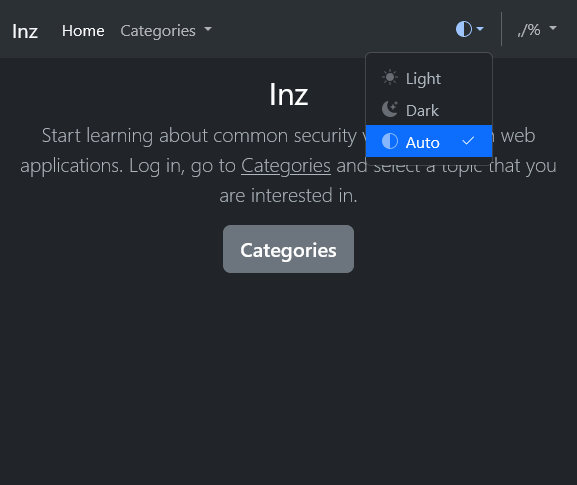
\includegraphics[width=\textwidth]{img/manual-theme-auto.png}
        \caption{Automatic theme - dark}
        \label{fig:manual-theme-auto}
    \end{subfigure}
    \hfill
    \begin{subfigure}{0.48\textwidth}
        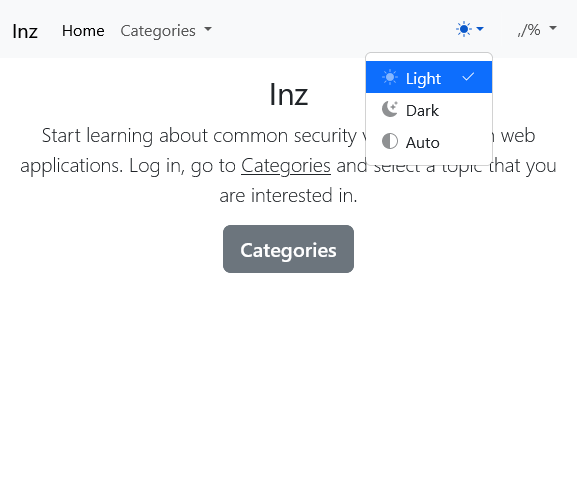
\includegraphics[width=\textwidth]{img/manual-theme-light.png}
        \caption{Light theme}
        \label{fig:manual-theme-light}
    \end{subfigure}
    \caption{Theme selection dropdown}
    \label{fig:manual-theme}
\end{figure}

\subsection{Account creation}
\label{chap:account-creation}

To access all features of the system a user account is required. Without it flag submission and later stages of solving tasks are impossible.

The account can be created on the \textit{Register} page which can be accessed from the home page as shown on Fig. \ref{fig:manual-home} or by clicking \textit{Create an account} on the login page. On that page the desired username and password have to be filled into the input fields. The password has to be between 8 and 64 characters long. To prevent mistakes in the password it has to be entered twice. If the passwords do not match the browser will prevent form submission and display an appropriate error.

The registration may fail if there already exists an account with the provided username. In such case a different username should be used.

\begin{figure}
    \centering
    \begin{minipage}{0.48\textwidth}
        \centering
        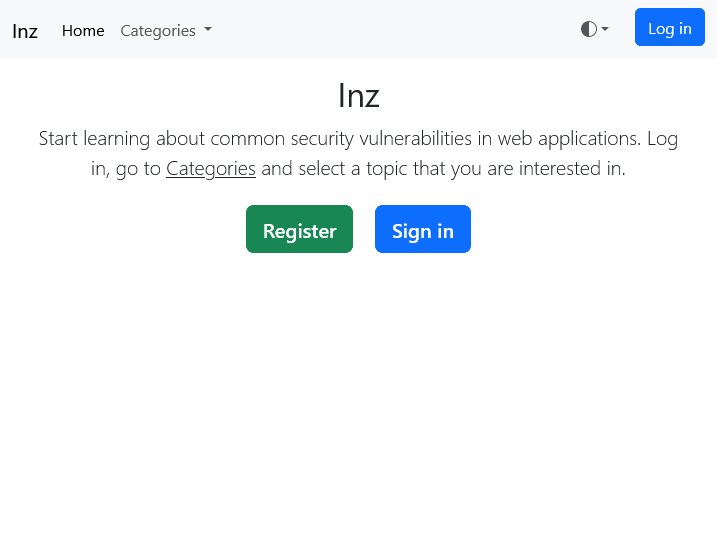
\includegraphics[width=\textwidth]{img/manual-home.png}
        \caption{Home page - logged out.}
        \label{fig:manual-home}
    \end{minipage}
    \hfill
    \begin{minipage}{0.48\textwidth}
        \centering
        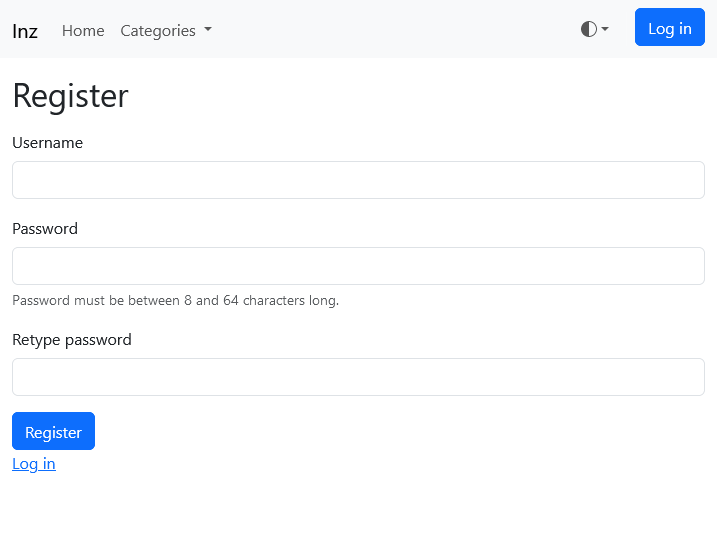
\includegraphics[width=\textwidth]{img/manual-registration.png}
        \caption{The registration page.}
        \label{fig:manual-registration}
    \end{minipage}
\end{figure}

\subsection{Logging in}

To use the account created in \ref{chap:account-creation} one has to log in into the account. To do that the user has to submit their username and password using a form on the login page (shown on Fig. \ref{fig:manual-login}). The page can be accessed by clicking a button in the navbar, a button on the home page or a link on the registration page.

\begin{figure}
    \centering
    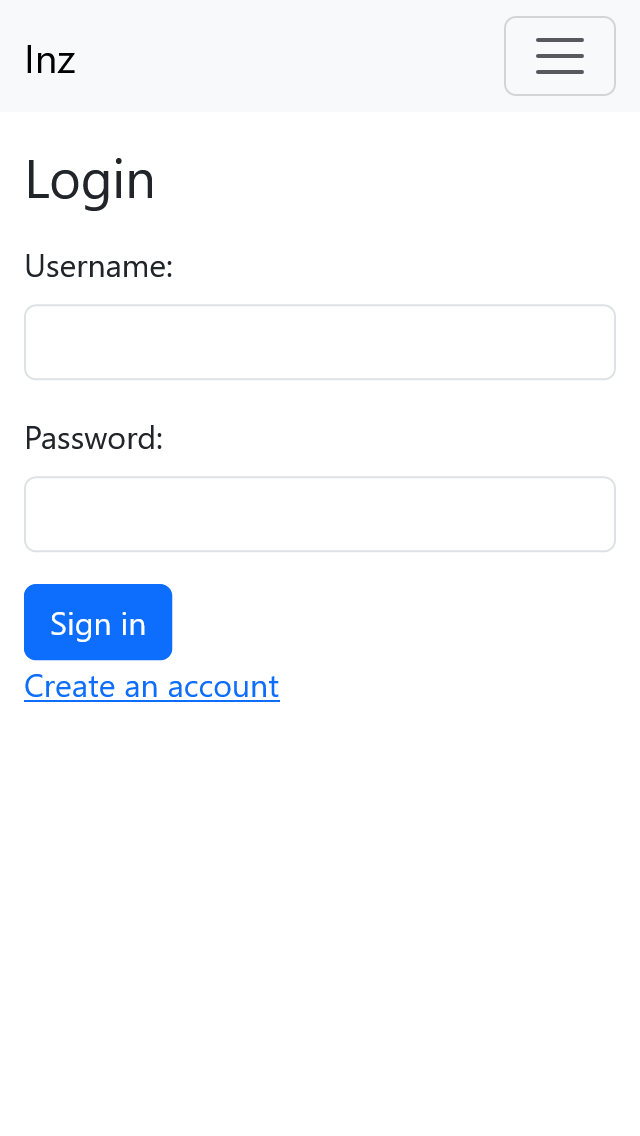
\includegraphics[width=0.4\textwidth]{img/manual-login.png}
    \caption{Login page viewed on mobile}
    \label{fig:manual-login}
\end{figure}

\subsection{Logging out}

A logged-in user can log out using the \textit{Log out} button in the dropdown appearing after the username in upper right corner is clicked. The dropdown is presented on Fig. \ref{fig:manual-home-dropdown-user}.

\begin{figure}
    \centering
    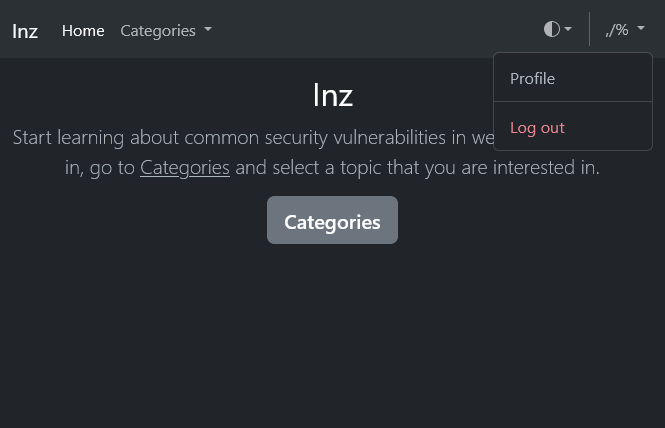
\includegraphics[width=\textwidth]{img/manual-home-dropdown-user.png}
    \caption{Username dropdown on home page for a regular user.}
    \label{fig:manual-home-dropdown-user}
\end{figure}

\subsection{Account management}

The profile page (\texttt{/profile}) shown on Fig. \ref{fig:manual-profile} is available for logged-in users through a link in the navbar (see Fig. \ref{fig:manual-home-dropdown-user}). This page allows changing the account password. To change the password one has to provide their current password and enter the new one two times. After submitting the form the system will show a message informing about the success or failure of the operation. Password change does not invalidate existing sessions.

\begin{figure}
    \centering
    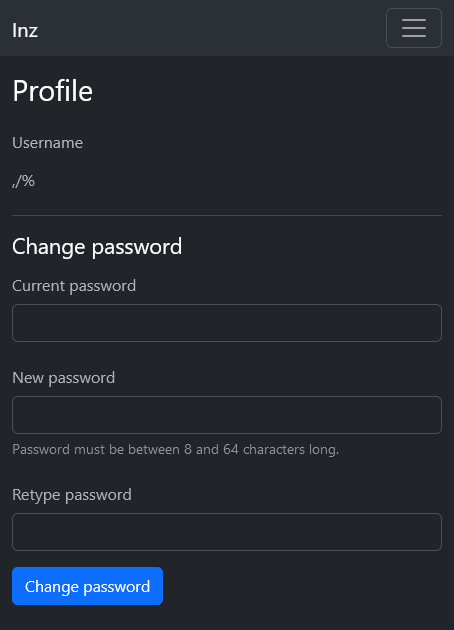
\includegraphics{img/manual-profile.png}
    \caption{Profile page in a narrow window.}
    \label{fig:manual-profile}
\end{figure}

\subsection{Browsing categories}

Categories in the system describe classes of vulnerabilities. A list of available categories can be accessed from the \textit{Categories} dropdown in navbar and from the \textit{Categories} (\texttt{/categories}) page. Both lists, presented on Fig. \ref{fig:manual-categories}, contain names of the categories which link to appropriate category pages.

\begin{figure}
    \centering
    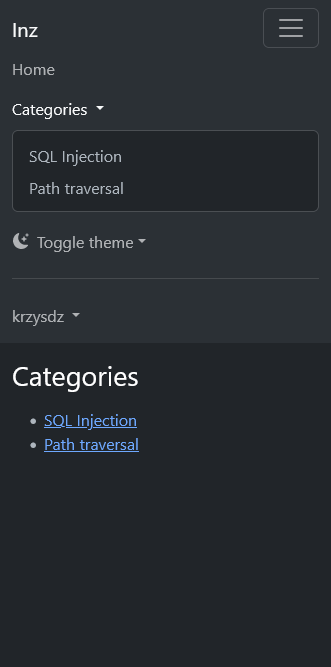
\includegraphics[width=0.5\textwidth]{img/manual-categories.png}
    \caption{Categories page with the categories dropdown open, viewed on mobile.}
    \label{fig:manual-categories}
\end{figure}

Category pages describe classes of vulnerabilities, why these exist and how they can be avoided. Additionally, on the bottom of each category page there is a list of related tasks which demonstrate examples of such issues.

\subsection{Tasks}

Tasks show specific examples of vulnerabilities. Each task contains a link to a challenge website which has to be exploited. The process will look differently for each challenge. As a result of a successful attack the user should obtain a flag. The flags should follow the \texttt{flag\{xxx\}} scheme unless specified otherwise in the task description. Tasks can contain hints which may help in case of problems when solving the linked challenge. The hints are collapsed by default to avoid spoilers and can be uncovered by clicking them.

Once the flag is found it should be submitted on the task page. Users who are not logged in will be prompted to log in as demonstrated on Fig. \ref{fig:manual-task-anon}. The form is shown only if the challenge is not solved as presented on Fig. \ref{fig:manual-task-user}. After a successful submission a message and a question appear instead of the form.

The second step of completing a task is answering a question like the one presented on Fig. \ref{fig:manual-task-solved}. Questions are related to the challenge and usually concern avoiding the problem or fixing it. There are multiple answers, each of which can be marked as true by marking the checkbox next to it. Conversely, if an answer is thought to be false the checkbox should be left empty. Finally, the answers should be sent by clicking the \textit{Submit} button.

If the question has been answered the checkboxes are disabled and reflect user's choices. Answers correctly marked as true or false are displayed in green, while incorrect are shown in red. Additionally, the true answers are listed on the bottom of the page. Below some answers an explanation may appear which expands on the answer. An example of this behaviour with an incorrectly marked first answer is presented on Fig. \ref{fig:manual-task-answered}.

Selected incorrect answers may contain additional challenges. Below these answers a link to the challenge will appear. These challenges are modified versions of the original challenge. After solving such challenge the obtained flag should be submitted using a form below the answer. If the additional challenge is solved a success message will replace the form as can be seen on figures \ref{fig:manual-task-answered} and \ref{fig:manual-task-complete}.

The whole process of solving a task can be observed on Fig. \ref{fig:manual-task}.

\begin{figure}
    \centering
    \begin{subfigure}{0.48\textwidth}
        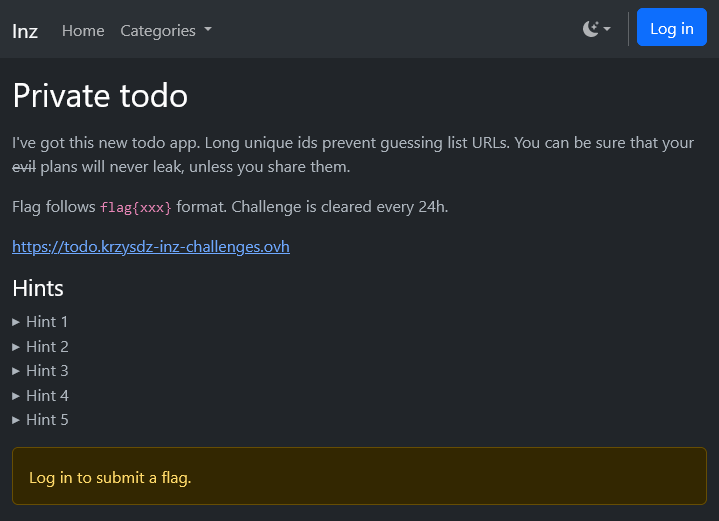
\includegraphics[width=\textwidth]{img/manual-task-anon.png}
        \caption{viewed while logged out}
        \label{fig:manual-task-anon}
    \end{subfigure}
    \hfill
    \begin{subfigure}{0.48\textwidth}
        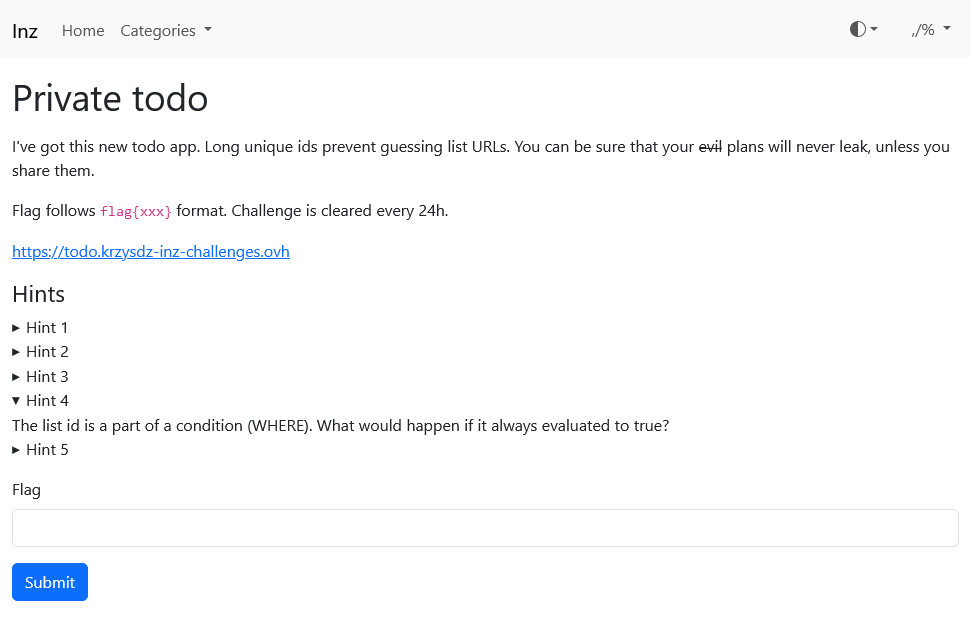
\includegraphics[width=\textwidth]{img/manual-task-user.png}
        \caption{viewed by user}
        \label{fig:manual-task-user}
    \end{subfigure}

    \begin{subfigure}{0.48\textwidth}
        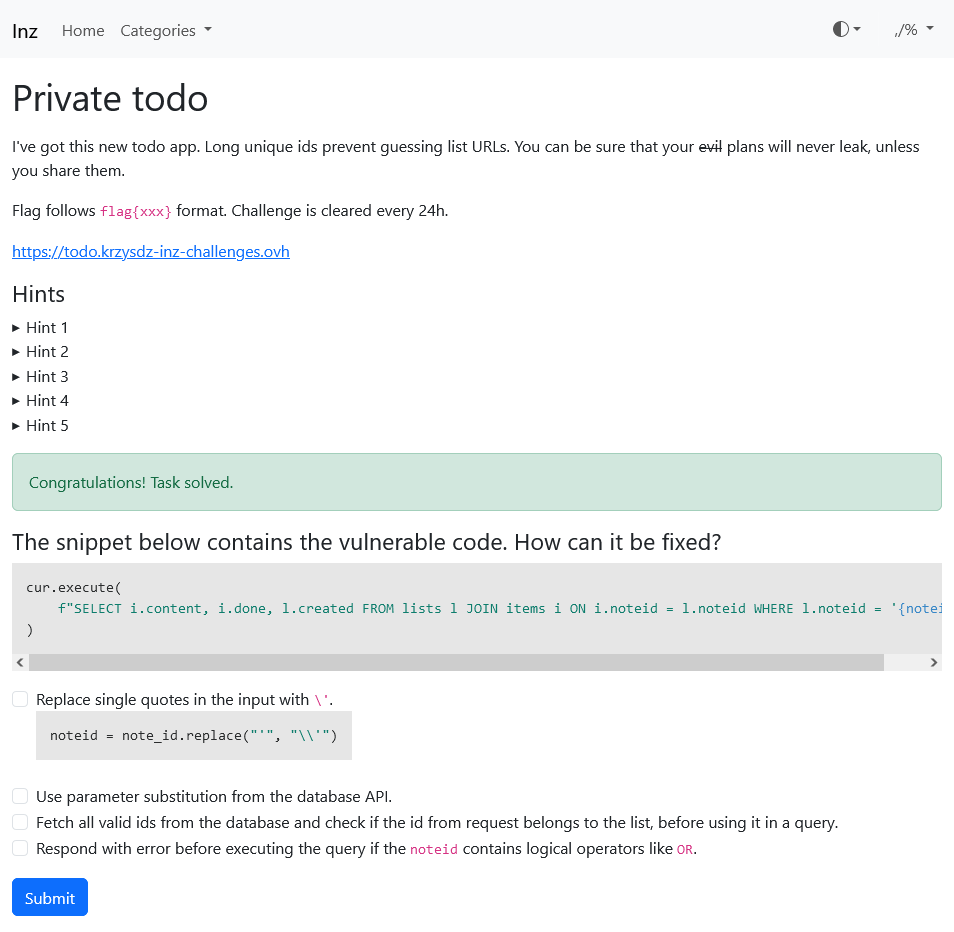
\includegraphics[width=\textwidth]{img/manual-task-solved.png}
        \caption{main challenge solved}
        \label{fig:manual-task-solved}
    \end{subfigure}
    \hfill
    \begin{subfigure}{0.48\textwidth}
        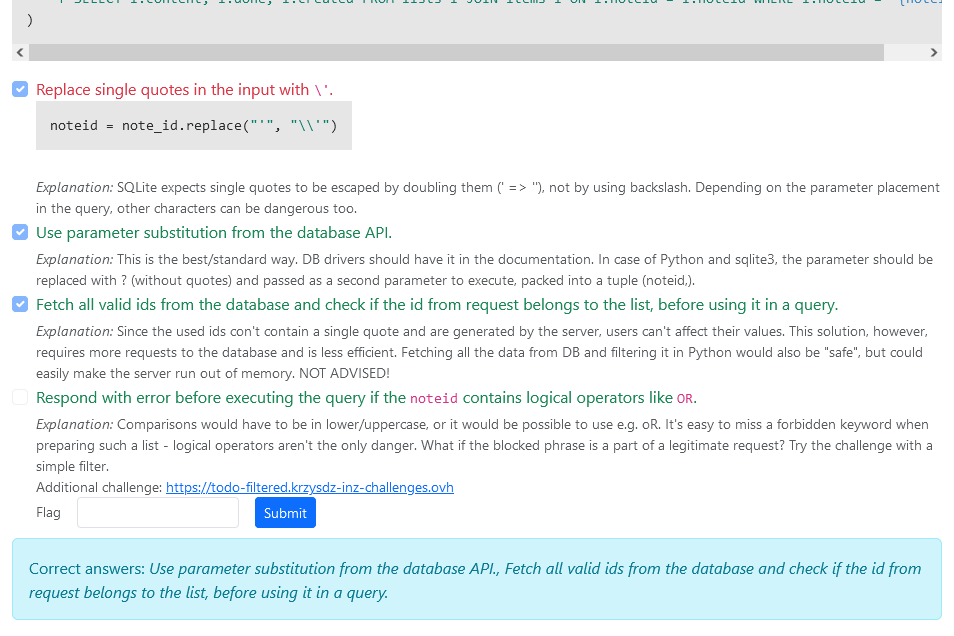
\includegraphics[width=\textwidth]{img/manual-task-answered.png}
        \caption{question answered, correct answers FTTF}
        \label{fig:manual-task-answered}
    \end{subfigure}

    \begin{subfigure}{0.7\textwidth}
        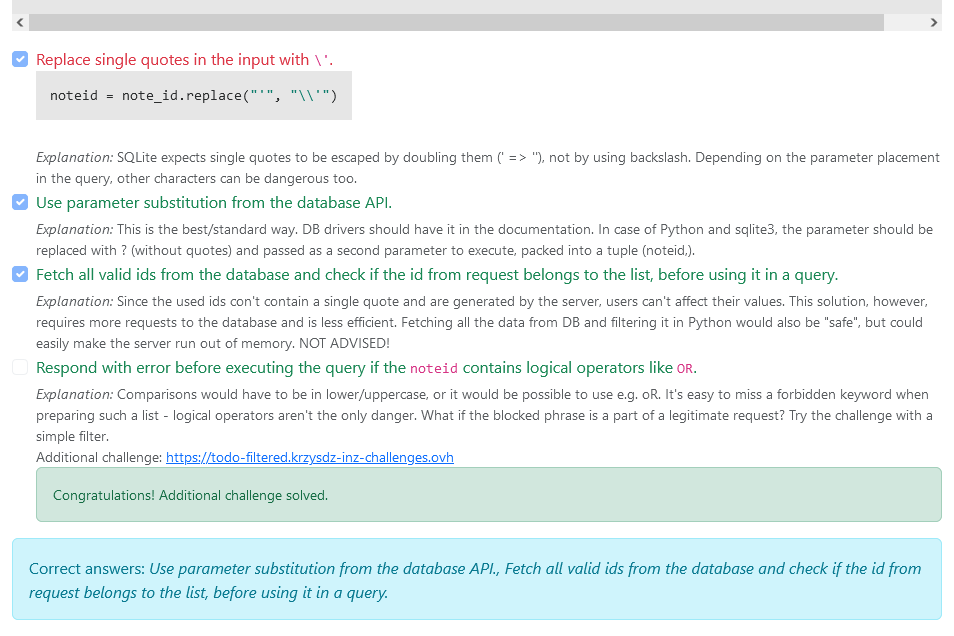
\includegraphics[width=\textwidth]{img/manual-task-complete.png}
        \caption{additional challenge solved}
        \label{fig:manual-task-complete}
    \end{subfigure}
    \caption{Task page at different stages of completion.}
    \label{fig:manual-task}
\end{figure}

\section{System administration}
\label{chap:system-administration}

The system is managed using and administrator panel \texttt{/admin}. It can be accessed from the dropdown in upper-right corner which is presented on Fig. \ref{fig:manual-admin-dropdown}. JavaScript is strictly required for all functionalities of the panel. There are three tabs for different categories of administrative capabilities.

\begin{figure}
    \centering
    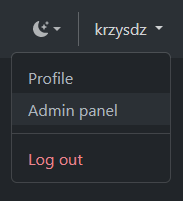
\includegraphics{img/manual-admin-dropdown.png}
    \caption{Dropdown with admin panel link.}
    \label{fig:manual-admin-dropdown}
\end{figure}

\subsection{Managing users}

The \textit{Users} tab presented on Fig. \ref{fig:manual-admin-users} offers basic account management features. In this tab a list of users registered in the system is presented. Next to each username their role is displayed. Finally, in the third column there are two action buttons. The first one changes user role from \texttt{user} to \texttt{admin} or the other way. The second one can be used to delete a user account. The list contains at most 10 entries. Pagination buttons below the table can be used to display another page of users.

\begin{figure}
    \centering
    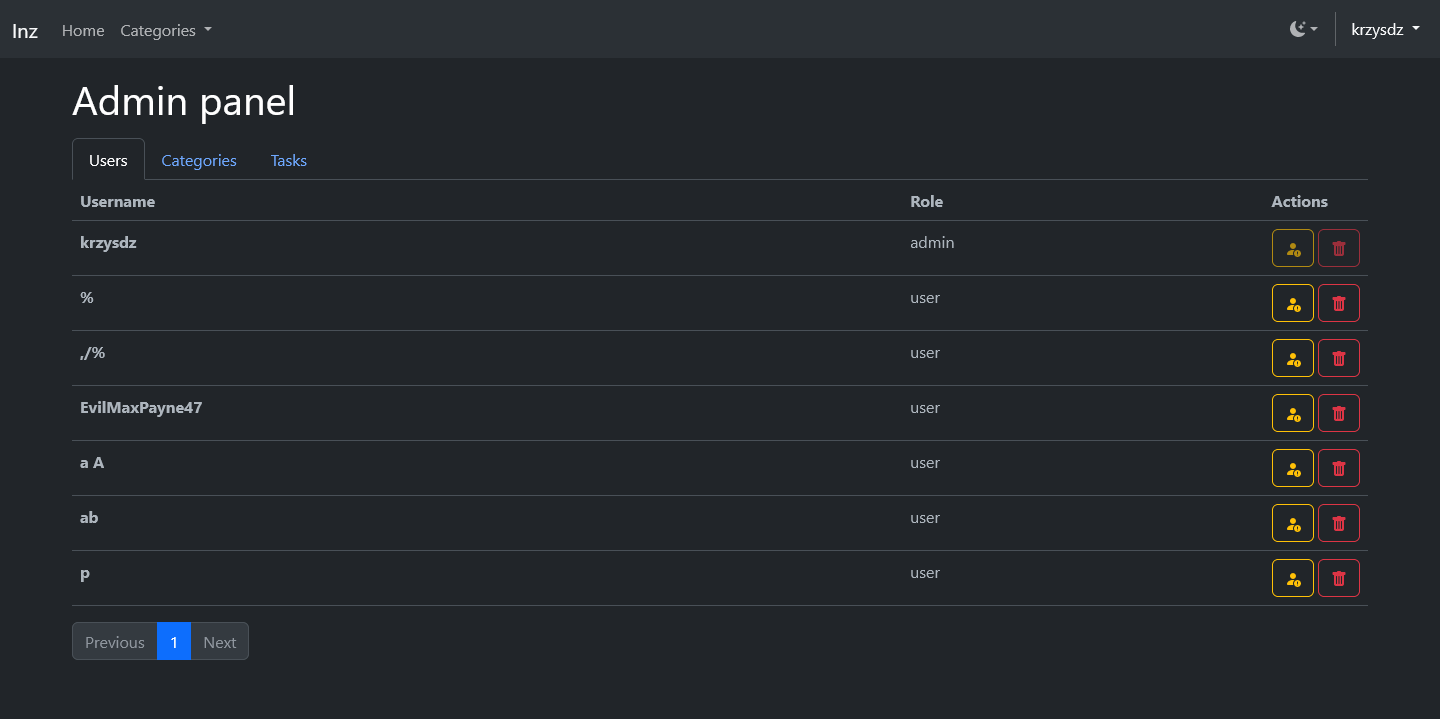
\includegraphics[width=\textwidth]{img/manual-admin-users.png}
    \caption{Users tab in admin panel.}
    \label{fig:manual-admin-users}
\end{figure}

\subsection{Managing categories}
\label{ssec:managing-categories}

The next tab \textit{Categories} allows creating and editing category pages. All existing categories are displayed as collapsed accordion items. Clicking on them opens a preview of the category description with an \textit{Edit category} button at the bottom. The categories tab with a single category expanded and an editor open is presented on Fig. \ref{fig:manual-admin-edit-category}.

\begin{figure}
    \centering
    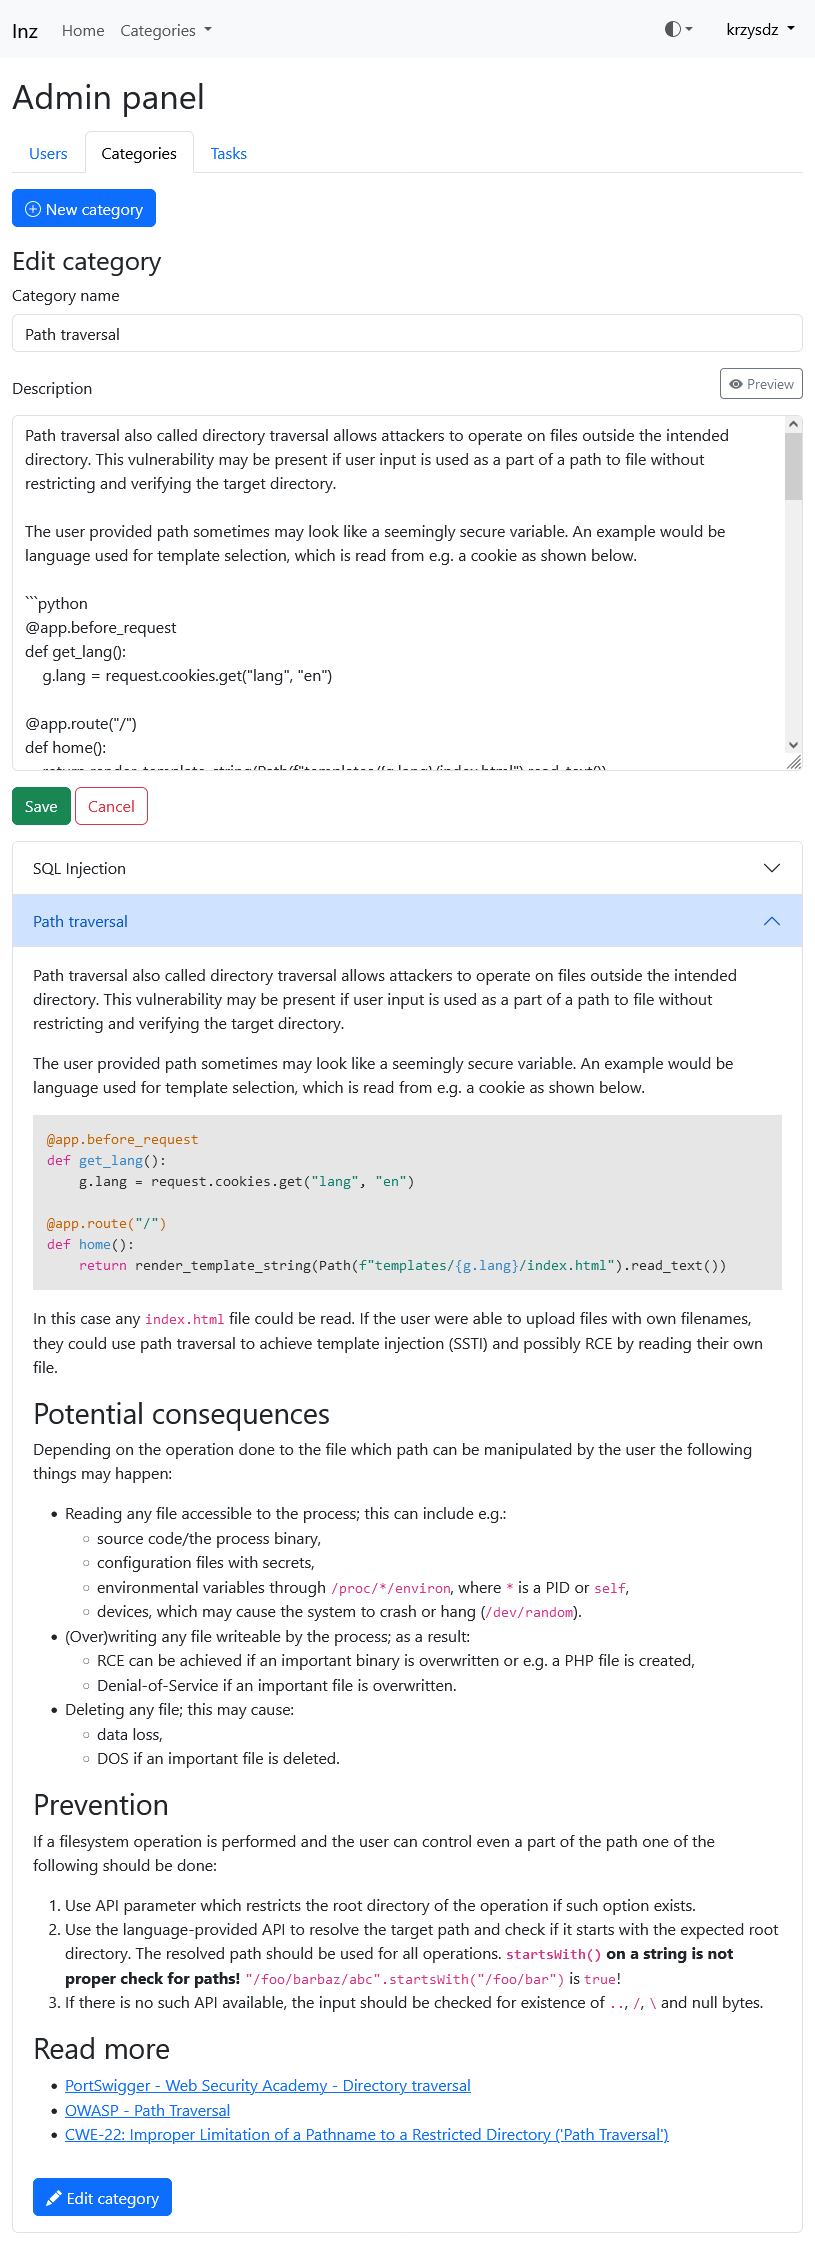
\includegraphics[width=0.539\textwidth]{img/manual-admin-edit-category.png}
    \caption{Categories tab with editor open and a category expanded.}
    \label{fig:manual-admin-edit-category}
\end{figure}

New categories can be created by clicking the \textit{New category} button at the top of the tab. The button opens a simple editor which can be used to create new categories. The name and description must be filled before creating the category using the \textit{Create} button. The name must use plain text, since it will always be escaped before displaying. The description should be entered using Markdown. To help with writing in Markdown a preview mode can be toggled by clicking the \textit{Preview} button on the right above the description input.

If the \textit{Edit category} button at the bottom of category description the editor will be populated with the stored details. The editor is the same as the one for new categories, but instead of the \textit{Create} button, a \textit{Save} button will appear.

Both creating a new category and editing an existing one causes reloading of the categories list. The description editor uses Marked for compiling Markdown content. The supported specification is listed at the bottom the discussion \href{https://github.com/markedjs/marked/discussions/1202}{markedjs/marked\#1202}.

\subsection{Managing tasks}
\label{ssec:managing-tasks}

The tab \textit{Tasks} show an overview of existing tasks and allows creating new. Like categories the existing tasks are listed as expandable accordion items. Fig. \ref{fig:manual-admin-add-task} presents the said tab and its options.

\begin{figure}
    \centering
    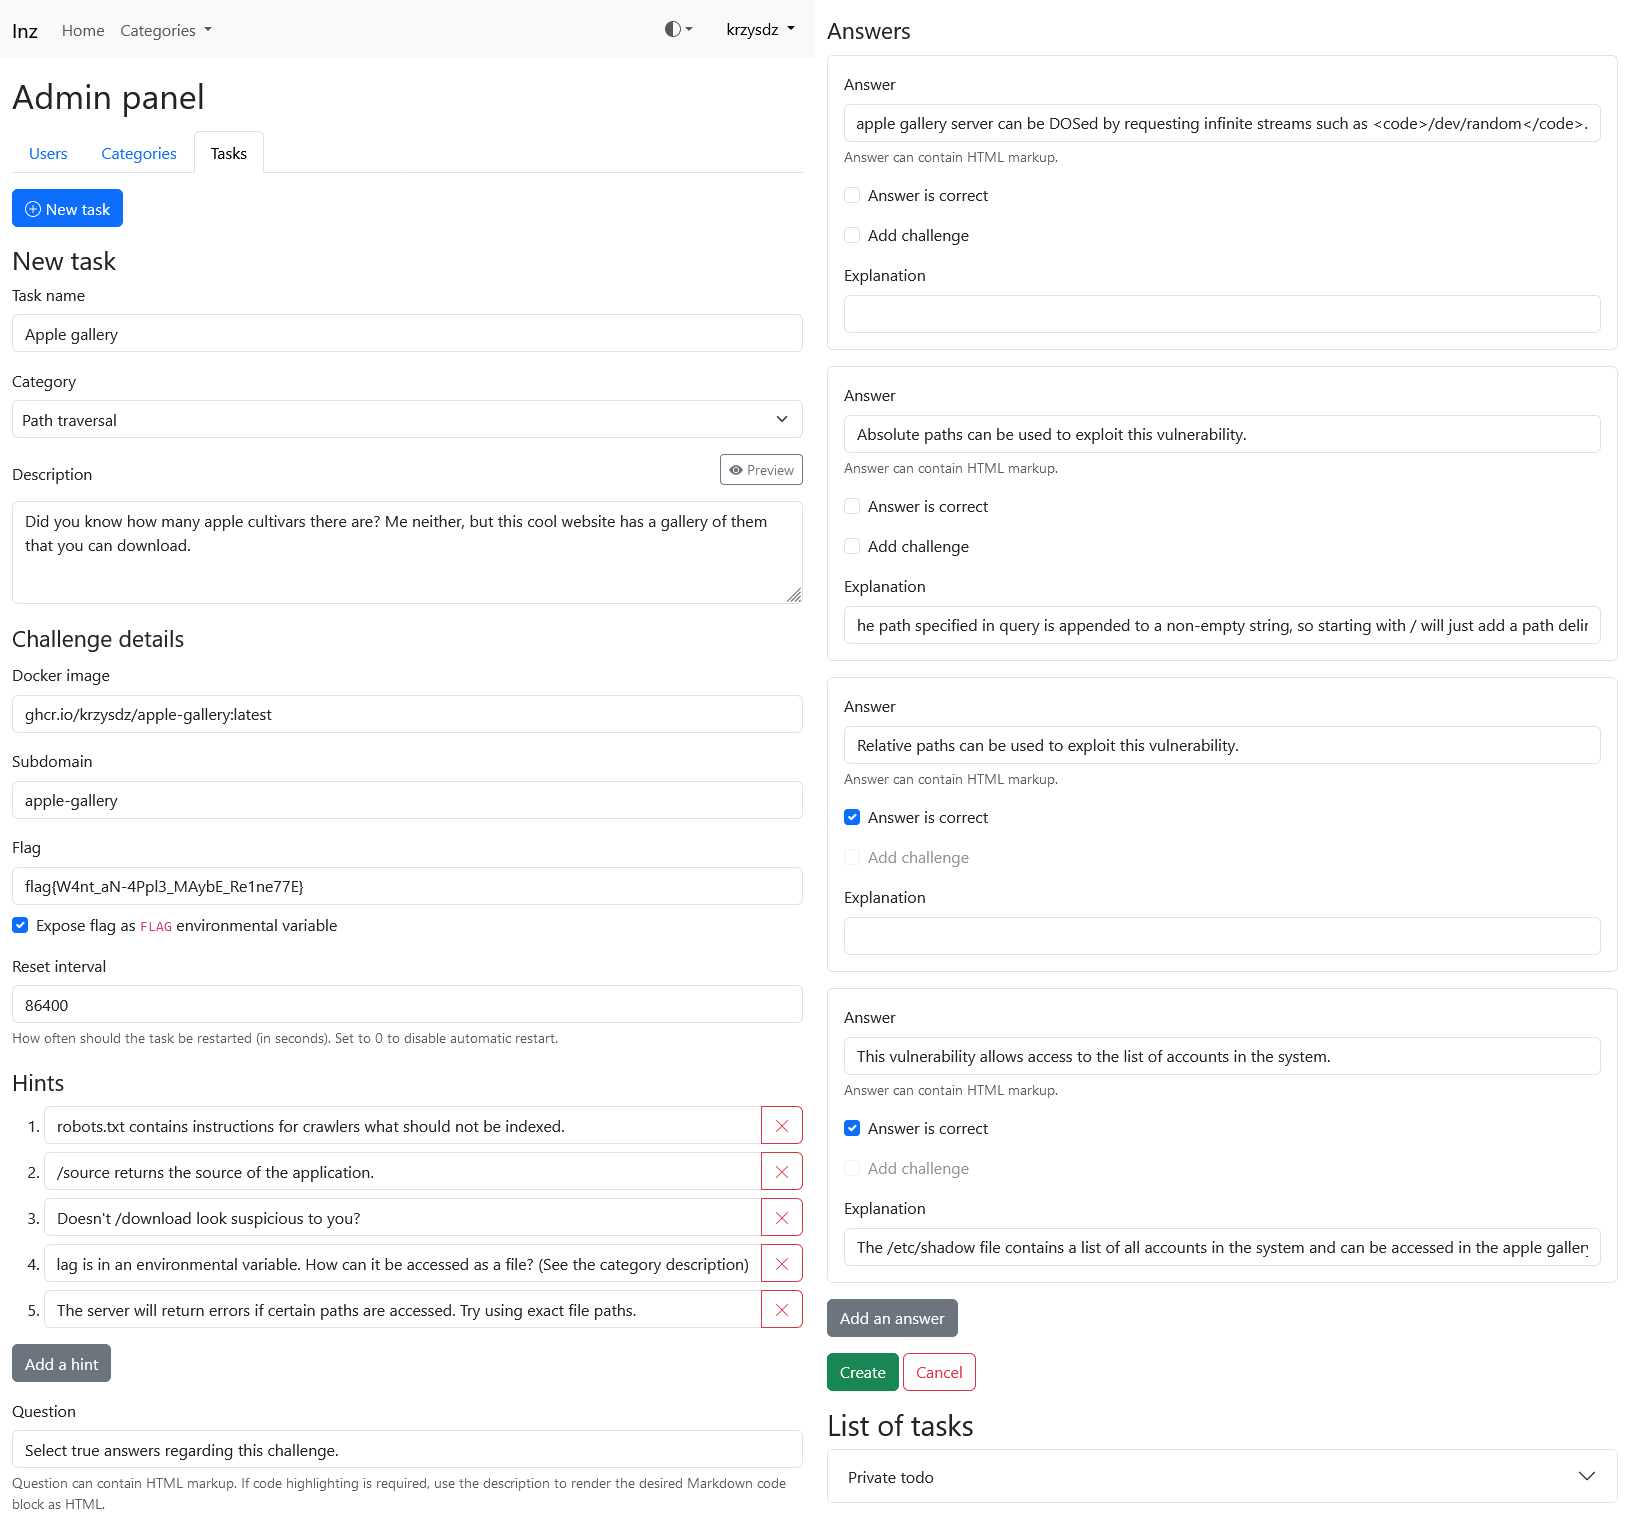
\includegraphics[width=\textwidth]{img/manual-admin-add-task-2col.png}
    \caption{Tasks tab with task editor open, presented in two columns.}
    \label{fig:manual-admin-add-task}
\end{figure}

New tasks can be added using a form which appears after clicking the \textit{New task} button at the top of the tab. The following data should be entered in the form:

\begin{itemize}
    \item \textbf{Task name:} The task name. It is displayed on the top of the task page and as a tile title on the bottom of relevant category page.
    \item \textbf{Category:} The category of vulnerabilities this task is assigned to. Must be chosen from one of the existing categories.
    \item \textbf{Description:} Task description displayed on the task page. The editor supports markdown and can be used the same way as the category description editor.
    \item \textbf{Challenge details:} The details for the main challenge. These options include:
    \begin{itemize}
        \item \textbf{Docker image:} Docker image to use for the challenge container. The image will be pulled after creating the task.
        \item \textbf{Subdomain:} Subdomain of the domain specified in the config file, which will be used to hosting the challenge.
        \item \textbf{Flag:} Flag which should be found by the users. Flags submitted by users will be compared to this value.
        \item \textbf{Expose flag as \texttt{FLAG} environmental variable:} Whether the flag should be exposed in the container as an environmental variable \texttt{FLAG}. This option can be used to avoid hardcoding flag values in challenge images.
        \item \textbf{Reset interval:} How often the challenge container should be removed and recreated. The value should be given in seconds. Set to 0 to disable automated restarts.
    \end{itemize}
    \item \textbf{Hints:} A list of hints for the main challenge. Hints are rendered inside a collapsed \mintinline{html}|<details>| tag on the task page, because they are supposed to contain \textit{spoilers}. New hints can be added by clicking \textit{Add a hint}. All hint inputs must be filled. The X button on the right of a hint input can be used to remove it. It is possible to create a task with no hints.
    \item \textbf{Question:} The question shown after solving the challenge. The question is rendered without escaping, so inline HTML can be used, but the content is placed inside an \mintinline{html}|<h4>| tag.
    \item \textbf{Answers:} These are the answers to the question from the field above. Additional answers can be added using the \textit{Add an answer} button. It is not possible to remove an answer. An answer has the following properties:
    \begin{itemize}
        \item \textbf{Answer:} The answer text that is presented to the users. The text is not escaped and can include HTML.
        \item \textbf{Answer is correct:} Whether the answer is correct and users are expected to check it.
        \item \textbf{Add challenge:} Shows an additional set of fields related to an extra challenge. \textbf{Available only if the answer is not marked as correct.}
        \item \textbf{Explanation:} An \textbf{optional} explanation that is shown after answering the question. It may underline the reasons why an answer is right or wrong.
        \item \textbf{Challenge details:} Challenge details for an additional challenge related to the answer. Options are the same as for the main challenge. \textbf{Shown only if the \textit{Add challenge} option is checked.}
    \end{itemize}
\end{itemize}

An expanded task accordion item presents the task properties. Challenge details other than the \textit{expose flag...} option are shown in collapsed \mintinline{html}|<details>|. Checkboxes next to answers indicate whether these answers are marked as correct. Optional explanations are shown in italics below respective answers.

\section{Security issues}

Secure design is an important part of the project. The target audience is expected to be or become experienced with exploitation, so the system had to be carefully created and must be responsibly managed.

\subsection{Project author's considerations}

Security of the system in a huge part depends on the main server design and implementation details.

\subsubsection{Data flow analysis}

The data sources provided by regular users are:
\begin{itemize}
    \item username set in the registration process - a string of at most 255 characters, always escaped in templates, inserted as \texttt{textContent} in admin panel, encoded with \mintinline{js}|encodeURIComponent()| in URLs,
    \item category name - a string (part of the URL), used for comparison in \texttt{\$match} stage of an aggregation pipeline as %TC:ignore
    \mintinline{js}|{ $match: { name: name } }|%TC:endignore
    ,
    \item task id and challenge id in challenge and quiz submissions - always a conversion to \texttt{ObjectId} is attempted, only the converted value is used later,
    \item flag in challenge solution submission - trimmed using \mintinline{js}|String.prototype.trim()| and compared using \mintinline{js}|===|,
    \item \texttt{answer[n]} properties in quiz submission - iterated from 0 to the number of answers in the task and compared to \mintinline{js}|"on"|.
\end{itemize}

The data coming from these sources is always used in a safe way. Data entered by administrators can be \textit{dangerous} by design, since they must be able to insert raw HTML and run any software using containers.

\subsubsection{Known vulnerabilities}

Express version used in the project depends on a vulnerable version of qs library (\href{https://www.cve.org/CVERecord?id=CVE-2022-24999}{CVE-2022-24999}). qs package is used in Express only if the \texttt{query parser} setting is set to \mintinline{js}|"extended"| or the \texttt{urlencoded} middleware's \texttt{extended} option is a truthy value. The \texttt{query parser} option is \mintinline{js}|"simple"| by default and the \texttt{urlencoded} middleware is created with \mintinline{js}|{ extended: false }|, so this vulnerability should not affect the project.

\subsection{Administrator's responsibilities}

Regardless of the project design it has to be configured and used properly so as not to introduce new security issues. System administrators should keep in mind the following warnings:

\begin{itemize}
    \item Challenges should use a different domain than the main website so that users who exploit a challenge will not be able to set cookies valid for the main domain.
    \item Special care must be taken when designing challenges, especially ones leading to RCE. Since challenges are running as Docker containers a misbehaving container can bring the whole system down. To provide isolation and limit resources use of \href{https://github.com/google/nsjail}{NsJail} is suggested.
\end{itemize}

\section{Covered categories of issues}

The design of the project separates the system from the content. Categories and tasks can be added at any time as described in sections \ref{ssec:managing-categories} and \ref{ssec:managing-tasks}. The example deployment covers some of the common security vulnerabilities found in web applications.

\subsection{SQL injection}

This category covers basics of SQL injection exploitation and prevention. Small code snippets and examples are provided to help users understand the reason behind this class of vulnerabilities. At the bottom of the description a \textit{Read more} section contains links to additional resources connected to this topic.

An example of a vulnerable application is presented in the \textit{Private todo} task. The target is a simple website offering to-do list creation and sharing. These lists are accessed using an \texttt{id} parameter, which is insecurely concatenated with the database query allowing for an injection attack. The question shown after solving the challenge presents the vulnerable line and answers show suggested methods of fixing the problem. One of them which proposes filtering some SQL keywords has an additional challenge.

\subsection{Path traversal}

The path traversal category gives a short overview of the vulnerability. The page presents a code which allows the user to read any file named index.html and execute it as template, therefore leaking some data and possibly introducing template injection. Consequences of this issue such as leaking any data the process has access to or even RCE with a short explanation are listed on this page. The prevention methods described in this category include using APIs which can restrict accessible directories, path verification after resolving them and characters which can be used for exploitation of this vulnerability.

The \textit{Apple gallery} task presents a simple gallery page with option to download albums. The download functionality is susceptible to path traversal and allows downloading almost any file from the system in a ZIP archive. The objective is reading a flag stored as an environmental variable using only path traversal. To help users the challenge exposes its own source code under \texttt{/source}, which is also mentioned in \texttt{/robots.txt}. The quiz presented after solving the challenge asks about the exploitation and gained access in this particular case.


\chapter{Internal specification}

The internal specification includes details regarding the system architecture and code which are useful for deep understanding of the platform's behaviour and introducing modifications.

% \section{Concept of the system}
% Let's just skip this section. I believe that the requirements contain enough information

\section{System architecture}

The system is managed by a server running on Node.js. As presented in Fig. \ref{fig:system-architecture}, this process manages the MongoDB database, challenge containers via Docker Engine API and the nginx proxy configuration. Challenges are run as Docker containers to enable easy configuration by just puling an appropriate image and each of them is bound to a different subdomain of a dedicated challenge domain thanks to the single proxy server.

\begin{figure}
    \centering
    % Text renders wrong without inkscapelatex=false
    \includesvg[inkscapelatex=false,scale=0.785]{img/system-architecture.svg}
    \caption{Visual representation of system architecture.}
    \label{fig:system-architecture}
\end{figure}

The nginx process is the only one exposed publicly. Other software can listen only on localhost for security reasons.

\section{Database structure}

The use of a NoSQL database allowed for a more flexible schema, based on the desired access to the data. A mix of embedded data model and normalized data model is used. The used database schema is presented in Fig. \ref{fig:db-schema}. Despite preferring the denormalized model, it was necessary to keep some relations between documents. This is achieved by storing fields with \texttt{\_id}s of referenced documents. There is also a relation between keys of embedded documents in the \texttt{users} collection, which are stored as stringified \texttt{ObjectId}s and documents from \texttt{tasks} and \texttt{challenges}. This relation, however, is not used in queries to the database, but managed completely by the server code.

There are two additional indexes:

\begin{itemize}
    \item a unique index on the \texttt{subdomain} field in the \texttt{challenges} collection to make sure that there are no duplicate subdomains,
    \item a unique index with a collation on the \texttt{name} field in the \texttt{categories} collection to accelerate case-insensitive search by category name and prevent duplicates.
\end{itemize}

The view \texttt{fullTasks} is a view collection on the \texttt{tasks}, which uses an aggregation pipeline to embed documents from the \texttt{challenges} collection using \texttt{\$lookup} where necessary. The pipeline is presented in Fig. \ref{fig:fullTasks-agg}.

\begin{figure}
    \centering
    % inkscapelatex=false, because the generated LaTeX file is invalid
    \includesvg[inkscapelatex=false,scale=0.87]{img/db-schema.svg}
    \caption{Visual diagram of the database schema.}
    \label{fig:db-schema}
\end{figure}

\section{Code organization}

The code is divided into ECMAScript modules. The main one is \texttt{index.js}, which imports all the other required modules, some external tools, configures and starts the server. Each module serves a separate function.

\subsection{Middleware}

Two modules are responsible for middleware functions. Middleware is a function called during request processing, which can act on the request and response objects and pass execution to functions declared later in the router stack.

One of them, \texttt{src/middleware.js}, contains general utility middleware functions:

\begin{itemize}
    \item \texttt{authenticated} - a middleware which returns 401 if the user is not logged in,
    \item \texttt{adminOnly} - a middleware which returns 403 if the user is not an administrator,
    \item \texttt{addCategoriesList} - a middleware executed before any routers, which fetches all category names and makes them available as response locals to use within templates.
\end{itemize}

The other module was separated, because it alters the request object and has an associated \texttt{.d.ts} typings file to help with type checking and code suggestions. It is \texttt{src/flash.js} and adds the following methods to each request object:
\begin{itemize}
    \item \mintinline{js}|flash(message, category = "info")| - a function which adds a message with category to a list of flash messages connected with the session,
    \item \texttt{getFlashedMessages(options)} - a function which returns the flashed messages with associated categories. This function can also filter the returned flashes by category. It is also available in response locals for direct use in templates.
\end{itemize}

The behaviour of this middleware is supposed to mimic the message flashing \href{https://flask.palletsprojects.com/en/2.2.x/quickstart/#message-flashing}{functionality} of the Flask framework.

\subsection{Routers}

The \texttt{index.js} module provides only the request handler for the root path \texttt{/}. Other paths are delegated to separate routers, which live inside modules under \texttt{src/routes}. The following paths are registered:
\begin{itemize}
    \item \texttt{/auth} handled by \texttt{authRouter} from the \texttt{auth.js} module. It serves the register, login and logout pages, as well as handles password change requests.
    \item \texttt{/profile} guarded by the \texttt{authenticated} middleware, handled by \texttt{profileRouter} from the \texttt{profile.js} module. It serves only the profile page.
    \item \texttt{/admin} guarded by the \texttt{authenticated} middleware, handled by \texttt{adminRouter} from the \texttt{admin.js} module.\\
    The router uses additional middleware \texttt{adminOnly} and \texttt{express.json()}. It renders only a single page - the admin panel. It provides a REST-like JSON API, which is used by a script on the admin panel page.
    \item \texttt{/category} handled by \texttt{categoryRouter} from the \texttt{category.js} module. It serves category pages with lists of related tasks and a category list page \texttt{/categories/}.
    \item \texttt{/task} handled by \texttt{taskRouter} from the \texttt{task} module. It serves task details pages and handles challenge and quiz submissions. All submissions are guarded with \texttt{authenticated}. The details page is handled separately for anonymous and other users as described in section \ref{chap:types-of-users}.
\end{itemize}

\subsection{Markdown parser}

To parse descriptions in Markdown the \href{https://marked.js.org/}{\texttt{marked}} parser is used together with syntax highlighting library \href{https://highlightjs.org/}{\texttt{highlight.js}}. Because the processing can take some time and the execution runtime is single-threaded, it is offloaded to a \href{https://nodejs.org/dist/latest-v19.x/docs/api/worker_threads.html}{worker thread}. The thread is terminated after a timeout passes to avoid blocking the thread pool \cite{bib:event-loop-explained,bib:event-loop-blocking}.

The first module responsible for this functionality \texttt{src/markedThread.js} listens to messages on \texttt{parentPort} and responds to them with an HTML string containing parsed Markdown.

The second module \texttt{src/markdown.js} exports a \texttt{processMarkdown} function, which manages the worker thread. It returns a \href{https://tc39.es/ecma262/multipage/control-abstraction-objects.html#sec-promise-objects}{\texttt{Promise}}, which is resolved after the worker sends the rendered string. If the worker emits an error event, the promise is rejected. After a specified time passes the worker is terminated and the promise rejected, unless it had finished successfully earlier.

\subsection{Database connection}

The module \texttt{src/db.js} does not export any functions. When it is imported it creates a \texttt{MongoClient} connected to the database server and opens the database specified in the configuration file. It calls then an \texttt{async} function \texttt{setupDb}, which prepares necessary indexes and views. Both the client (\texttt{client}) and database (\texttt{db}) are exported. All modules importing either exported variable reuse the same client connection.

\subsection{Challenge management}

Challenges are managed using functions from the \texttt{src/challenges.js} module. The module has the following functions:
\begin{itemize}
    \item \mintinline{js}|getChallengeContainers(all = false)| - returns challenge containers (only running, unless \texttt{all} is \texttt{true}). It relies on label \texttt{pl.krzysdz.inz.challenge-kind} being present.
    \item \texttt{startupChallenges()} - removes all nginx subdomain configuration files, stops and removes all challenge containers and calls \texttt{addChallenge} with each challenge document from the database.
    \item \mintinline{js}|addChallenge(challengeDoc, reload = false)| - verifies the image tag, then calls functions \texttt{startChallengeContainer} and \texttt{createNginxConfig}. If \texttt{reload} is \texttt{true}, calls a function responsible for reloading nginx configuration.
    \item \texttt{checkTag(challengeDoc)} - checks if the document contains an image with a tag. If there is no tag, \texttt{:latest} is appended to the image name. Returns the \texttt{challengeDoc} with corrected \texttt{taskImage} field.
    \item \texttt{startChallengeContainer(challengeDoc)} - pulls the image specified in the argument, stops and removes containers with the same name if they exist, creates a new container and starts it. If \texttt{resetInterval} is not 0, \texttt{setInterval} is created, which uses \texttt{restartChallengeContainer} to periodically restart the container.
    \item \texttt{restartChallengeContainer(port, challengeDoc)} - restarts the container specified in \texttt{challengeDoc}. This function is not exported and called only in interval, which is created after starting the container for the first time. It stops and removes the container including volumes, creates a new container reusing the same port and starts the new container.
    \item \texttt{createNginxConfig(subdomain, port)} - creates an nginx configuration file in \texttt{nginx/conf/subdomains} directory, which defines an HTTPS server proxying request made to the subdomain of domain specified in config to the specified port on localhost.
    \item \texttt{reloadNginx()} - executes the nginx binary with \texttt{-s reload} and prefix set to \texttt{./nginx} from the project directory to instruct the proxy to reload its configuration.
\end{itemize}

\section{Sequence diagrams}

Basic system functionality in a simplified form can be presented in form of UML sequence diagrams. Figures \ref{fig:seq-register}, \ref{fig:seq-login} and \ref{fig:seq-change-pass} demonstrate flows related to authentication and account management. The next three diagrams \ref{fig:seq-task}, \ref{fig:seq-task-flag} and \ref{fig:seq-task-answer} present operations connected with tasks. The diagrams are simplified, to avoid repeating the process of fetching task and checking user progress before rendering the page.

% Text in diagrams doesn't look good without inkscapelatex=false
% Too wide or positioned incorrectly

\begin{figure}
    \centering
    \includesvg[inkscapelatex=false]{uml/render/seq-register.svg}
    \caption{Registration sequence diagram.}
    \label{fig:seq-register}
\end{figure}

\begin{figure}
    \centering
    \includesvg[inkscapelatex=false]{uml/render/seq-login.svg}
    \caption{Logging in sequence diagram.}
    \label{fig:seq-login}
\end{figure}

\begin{figure}
    \centering
    \includesvg[inkscapelatex=false]{uml/render/seq-change-pass.svg}
    \caption{Password change sequence diagram.}
    \label{fig:seq-change-pass}
\end{figure}

\begin{figure}
    \centering
    \includesvg[inkscapelatex=false, scale=0.9]{uml/render/seq-open-solve-task.svg}
    \caption{Navigation and solving a task.}
    \label{fig:seq-task}
\end{figure}

\begin{figure}
    \centering
    \includesvg[inkscapelatex=false]{uml/render/seq-task-flag.svg}
    \caption{Submitting challenge flag.}
    \label{fig:seq-task-flag}
\end{figure}

\begin{figure}
    % Don't use inkscapelatex=false to render \ref, make font smaller manually
    \fontsize{10}{12}\selectfont
    \centering
    \includesvg[]{uml/render/seq-task-answer.svg}
    \caption{Answering task question.}
    \label{fig:seq-task-answer}
\end{figure}

Actions available for the administrators involve an additional participant - a script running in the browser which is responsible for managing the UI and communication with the server. Because the panel is not rendered on the server, the process of loading it is more complicated as can be seen in Fig. \ref{fig:seq-admin-load}. The most complicated operation is adding a new task. The flow is presented in Fig. \ref{fig:seq-admin-add-task} and requires interactions with even more system components.

\begin{figure}
    \centering
    \includesvg[inkscapelatex=false, scale=0.9]{uml/render/seq-admin-load.svg}
    \caption{Loading administrator panel.}
    \label{fig:seq-admin-load}
\end{figure}

\begin{figure}
    \centering
    \includesvg[inkscapelatex=false, scale=0.57]{uml/render/seq-admin-add-task.svg}
    \caption{Adding a new task.}
    \label{fig:seq-admin-add-task}
\end{figure}


%TC:envir minted [xx] xxx
\chapter{Verification and validation}

The solution was tested to ensure that it meets all the requirements and provides a bug-free experience.

\section{Testing procedure}

The testing was performed entirely manually. Features were tested as they were developed. The manual incremental approach was chosen due to time considerations. The project is rather small and the result of many operations is a UI rendered from an HTML template, which would make automated testing much more time consuming. Additionally the interface had to be visually inspected, so feature testing could be performed as a part of this procedure. Some features such as creating and restarting challenges were tested by either running small scripts or using them via the Node.js REPL and observing results in external tools.

\section{Requirements verification}

The verification of chapter \ref{chap:req-and-tools} requirements fulfilment.

\subsection{Verification of functional requirements}

\begin{enumerate}
	\item \textbf{Account creation}: There is an option to register a new account. Minimum password length is verified both on the client side and on server. It is impossible to register an account with the same username. Additionally the password has to be typed twice to prevent typos. Stored password is hashed and salted. Accounts are created with the \texttt{"user"} role. The functionality is available under \texttt{/auth/register}. \textbf{Requirement met completely.}

	\item \textbf{Signing in}: Possible through a login page, which is linked in the navbar and on the home page. The functionality is available under \texttt{/auth/login}. \textbf{Requirement met completely.}

	\item \textbf{Logging out}: Users can log out by clicking the logout button, which redirects to \texttt{/auth/logout}. \textbf{Requirement met completely.}

	\item \textbf{Changing password}: Password can be changed on the profile page \texttt{/profile}. The previous password as well as the new password typed twice are required. \textbf{Requirement met completely.}

	\item \textbf{Listing categories}: The list of categories is available in the \textit{Categories} dropdown and on the \texttt{/categories} page. \textbf{Requirement met completely.}

	\item \textbf{Displaying category}: Category pages are provided under \texttt{/category/<name>}. \textbf{Requirement met completely.}

	\item \textbf{Displaying task}: All task properties specified in the requirements are displayed on task pages \texttt{/task/<id>}. \textbf{Requirement met completely.}

	\item \textbf{Solving challenge}: Logged in users can solve tasks as described in the requirements. \textbf{Requirement met completely.}

	\item \textbf{Answering quiz}: Users who have solved the task challenge can answer the quiz. After answering the correctly marked answers are displayed in green. A summary of correct answers is displayed below the quiz. \textbf{Requirement met completely.}

	\item \textbf{Administrator panel}: Administrator panel is available only for administrators as \texttt{/admin} page. \textbf{Requirement met completely.}

	\item \textbf{Listing users}: The list of users is available under the \textit{Users} tab in the admin panel. The list can also be accessed as JSON as a response to \texttt{GET} request to \texttt{/admin/users} with \texttt{page} and \texttt{size} query parameters. \textbf{Requirement met completely.}

	\item \textbf{Changing user permissions}: User role can be toggled by clicking a button next to the user on the users list. \textbf{Requirement met completely.}

	\item \textbf{Deleting user}: An account can be removed by clicking the red bin icon next to the user on the users list. \textbf{Requirement met completely.}

	\item \textbf{Creating category}: Categories can be created using a form in the \textit{Categories} tab in the admin panel. A \textit{Preview} button can be clicked to toggle between the description input and the preview of rendered HTML. \textbf{Requirement met completely.}

	\item \textbf{Editing category}: Categories can be edited by clicking the \textit{Edit category} button below the category description in the admin panel. The same editor is used for modifying categories as for creating them. \textbf{Requirement met completely.}

	\item \textbf{Creating task}: Tasks can be added as described in the requirements in the \textit{Tasks} tab of the admin panel. \textbf{Requirement met completely.}

	\item \textbf{Starting challenges}: When a task is added, the system automatically starts related challenges. Challenges containers and related nginx configuration are also configured while starting the server. \textbf{Requirement met completely.}
\end{enumerate}

\subsection{Verification of non-functional requirements}

\begin{enumerate}
	\item \textbf{Responsiveness}: The interface has been tested on multiple screen sizes and devices as well as in-browser zoom. The tested native resolutions include: $1920 \times 1080$ (24 in - desktop), $1440 \times 900$ (19 in), $1336 \times 768$ (15.6 in - laptop) and $2400 \times 1080$ (6.67 in - smartphone). Additional screen sizes were tested using the \textit{responsive mode} option in Firefox developer tools. No issues were found during the visual inspection although some answers may cause the viewport to scroll on small screens if they contain specific HTML. \textbf{Requirement met completely.}

	\item \textbf{Accessibility}: There are no accessibility errors in the webhint scan results run from Firefox developer tools. Warning are related to contrast especially in code blocks in light mode. The accessibility results of the scan are presented on Fig. \ref{fig:verify-webhint}. \textbf{Requirement met completely.}

	\item \textbf{Visual consistency}: Styles from the Bootstrap library were used. Additional style sheets follow the Bootstrap colours. Code highlighting follows the theme variant changes (light/dark) and in both modes an appropriate variation of the Panda Syntax theme is used. \textbf{Requirement met completely.}

	\item \textbf{Page load performance}: 98 points performance score in PageSpeed Insights mobile test. Test results are presented on Fig. \ref{fig:verify-perf}. \textbf{Requirement met completely.}

	\item \textbf{Compatibility}: The user interface has been verified to display and work correctly on Firefox, Chrome and Tor Browser (based on Firefox ESR) on Windows, Firefox on Ubuntu and Firefox on Android. Client-side form verification errors are not displayed on Firefox for Android due to \href{https://bugzilla.mozilla.org/show_bug.cgi?id=1510450}{bug 1510450}. Bootstrap dropdowns do not work without JavaScript, so it is impossible to logout or access the profile page with JS disabled. Changing page theme also requires JavaScript, but it is not a core functionality. \textbf{Requirement met partially.}
\end{enumerate}

\begin{figure}
	\centering
	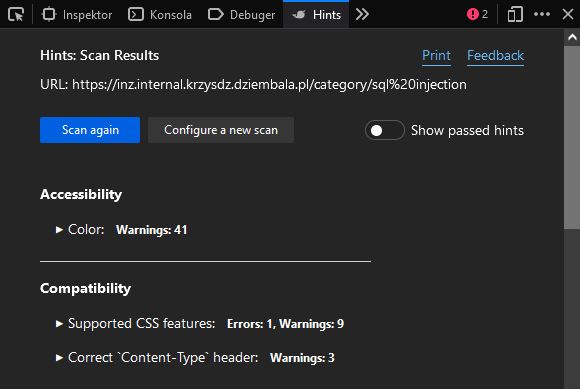
\includegraphics{img/verify-webhint.png}
	\caption{Webhint scan warnings and errors}
	\label{fig:verify-webhint}
\end{figure}

\begin{figure}
	\centering
	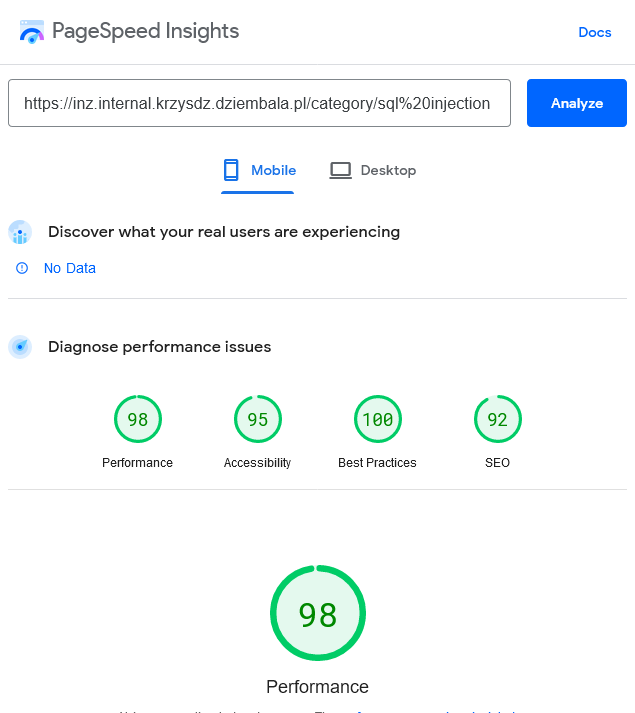
\includegraphics[width=\textwidth]{img/verify-performance-mobile.png}
	\caption{PageSpeed Insights mobile test results}
	\label{fig:verify-perf}
\end{figure}

\section{Detected and fixed bugs}

Most issues were found while writing new features and immediately fixed as a part of adding these features. Some issues, however, slipped through unnoticed and were found and patched separately.

\subsection{Containers were not started at launch if stopped}

If for some reason (eg. OS restart) challenge containers were stopped while starting the server, these would not be removed and their recreation and start would fail.

The problem was fixed in \href{https://github.com/krzysdz/inz/commit/9fd9017ce994f577233ce0544bbd0cf1df3e0e55}{\texttt{9fd9017}} by ignoring \textit{"container already stopped"} errors when stopping a container.

\subsection{Cookies not set in production}

Cookies were not sent in responses if \mintinline{bash}|NODE_ENV="production"| environmental variable was set. The problem happened, because Express does not send cookies marked as \texttt{secure} if the request was not made with HTTPS. While nginx terminates the external connections with HTTPS, it uses plain unencrypted HTTP to communicate with the server which recognises it as an insecure protocol.

This problem was fixed in \href{https://github.com/krzysdz/inz/commit/94ca9c4124954c94c9fe8e27dc59305aa59b31ad}{\texttt{94ca9c4}} by setting appropriate headers in the proxy
\begin{minted}{nginx}
proxy_set_header X-Forwarded-Proto $scheme;
proxy_set_header X-Forwarded-For $remote_addr;
\end{minted}
and telling Express to trust the proxy
\begin{minted}[breaklines]{js}
// In production the only way is through nginx, which sets X-Forwarded-For to $remote_addr
if (process.env.NODE_ENV === "production") app.set("trust proxy", true);
\end{minted}
With this change Express recognises HTTPS connections to the proxy as secure and sends cookies in responses.

\subsection{Unsolved question on task page was escaped}

Task questions should support HTML content and be inserted into template without escaping. In commit \href{https://github.com/krzysdz/inz/commit/b5ae1b16e9be6060b43f28dbb56b090bfb46dd98}{\texttt{b5ae1b1}} support for HTML in questions and answers was added, but this particular place has been overlooked.

The problem was fixed in \href{https://github.com/krzysdz/inz/commit/91128c835889ac0429b478d03c6992541fcdd5c3}{\texttt{91128c8}} with a single line patch:
\begin{minted}[]{diff}
- <h4><%= locals.task.question %></h4>
+ <h4><%- locals.task.question %></h4>
\end{minted}

\subsection{Flag not set as an environmental variable on start}
\label{chap:bug-env-not-set-start}

If \texttt{flagInEnv} was \texttt{true}, the flag would be exposed as an environmental variable when restarting the container, but not after creating it for the first time or restarting the server.

In this instance the problem was fixed in \href{https://github.com/krzysdz/inz/commit/99a0035c61de55ddd7203e7ced1e9fc554959f24}{\texttt{99a0035}} by adding the missing \texttt{Env} option to the \texttt{createContainer} call in \texttt{startChallengeContainer}.

\subsection{Flag not set as an environmental variable for the main challenge}

The \texttt{flagInEnv} option was not saved for the main challenge. The problem was discovered when testing the fix for \ref{chap:bug-env-not-set-start}.

The problem was fixed in \href{https://github.com/krzysdz/inz/commit/f934efb0c50f0156d73bd78fcfcd6a12b5943b1e}{\texttt{f934efb}} by passing the missing option.

\subsection{Task creation fails without additional challenges}

If there were no additional challenges for the incorrect answers, task creation would fail, because \texttt{insertMany()} throws an error if an empty array is passed. There was an empty array check, but it had been implemented incorrectly.

The problem was fixed in \href{https://github.com/krzysdz/inz/commit/f934efb0c50f0156d73bd78fcfcd6a12b5943b1e}{\texttt{f934efb}} by verifying the truthiness of array length instead of the array itself:
\begin{minted}[tabsize=4, obeytabs]{diff}
-		const subChallengeResult = answerChallengeDocs
+		const subChallengeResult = answerChallengeDocs.length
			? await challengesCollection.insertMany(answerChallengeDocs, {
				session,
			})
\end{minted}

\subsection{HSTS header set three times per response}

The \texttt{Strict-Transport-Security} header was sent 3 times with each response. The problem was detected by one of external tools while checking compatibility, accessibility and HTTPS configuration.

The problem was fixed in \href{https://github.com/krzysdz/inz/commit/eec703c98ecb6720c3c2eb0ceee36ca3d7da8aa2}{\texttt{eec703c}} by setting the \texttt{hsts} option of the \href{https://helmetjs.github.io/}{Helmet} middleware to \texttt{false} and removing an \texttt{add\_header} directive from the main configuration, since the shared \texttt{ssl\_common.conf} configuration already contains one.


\chapter{Conclusions}

The project meets all the requirements listed in chapter \ref{chap:req-and-tools}. The created project allows creating vulnerability descriptions with managed CTF tasks and quizzes. Unlike the alternatives presented in section \ref{sec:existing-solutions} it combines the user interface and challenge management in a single package. Other features unique to this solution are the optional additional challenges related to quiz answers and the per-answer explanations available after solving the quiz. It lacks, however, versatility as it has been developed with web application security in mind.

\section{Future development ideas}

Although the project is usable and demonstrates a general idea there is still an area for improvements. This section lists some propositions for future project development.

\subsection{More content}

The most valuable part of the system for regular users is the content - description of vulnerabilities and tasks. The currently offered examples just scratch the surface of web application security. Expanding the topics, adding more diverse tasks and introducing new categories certainly would enrich the user experience. Broadening the repertoire could make the service useful to a wider audience as well as present the vulnerabilities in more details.

Increasing the number of tasks in a single category with different difficulty levels creates a risk of a less legible and usable category pages and could discourage users less experienced with those categories. To avoid that problem the tasks could be tagged with a difficulty level and ordered by it, so everyone will be able to choose what best matches their abilities and ambitions.

\subsection{Better task management}

Current task management is restricted to task creation, which is rather complicated and involves filling a complex form properly in one try. This aspect can be greatly improved by introducing the following changes:
\begin{itemize}
	\item allow editing existing tasks - ideally the edits would be applied separately to each part (name, description, question, challenge, etc.) of the task to reduce the complexity of changes and make the implementation simpler; this functionality could be used to fix mistakes in the text or update challenges if the image is fixed to a specific version,
	\item task drafts - tasks hidden from users, which may not have all the required fields filled,
	\item health checks and container status - monitoring the status of a challenge container and periodical checks of the application inside could help diagnose issues and prevent users accidentally or purposefully taking the tasks down; could be paired with an alert system to administrators and automated restarts,
	\item forced manual restart - in case a task is down or vandalized and the automatic reset is not going to happen soon, the administrators should be able to force a challenge container reset,
	\item time to the next restart - when the challenge will be recreated from the initial state automatically, this could be also shown on the task page to users,
	\item importing from file - tasks could be imported from a JSON, YAML or other file to help with sharing task configurations between separate deployments,
	\item file attachments - files attached to tasks could be used to share source code to help users and would be useful if someone wanted to use the platform for demonstration of not web-related vulnerabilities.
\end{itemize}

\subsection{User overview for administrators}

To help with debugging possible issues user actions such as flag and answer submission could be logged, even if the flag is invalid. An overview of such events could be then checked by an administrator to verify the user findings, detect misconfigured challenges or hint the user, if for example they found a bait flag left by another user.

\subsection{Progress tracking}

The users can see their progress for a single task when they open it. A progress bar or a colour change could be added to task tiles on category pages to indicate whether a task has been solved and to what level (challenge solved, task answered, all challenges solved).

\subsection{Increasing user engagement}

User engagement could be improved by introducing a public scoreboard and therefore an element of competitiveness. However, publishing their own results should not be mandatory, so as not to discourage the privacy-focused or less confident users.


\backmatter

%\bibliographystyle{plain}  % bibtex
%\bibliography{biblio/biblio} % bibtex
\printbibliography           % biblatex
\addcontentsline{toc}{chapter}{Bibliography}

\begin{appendices}


\chapter{Index of abbreviations and symbols}

\begin{itemize}
	\item[CTF] Capture The Flag
	\item[SQL] Structured Query Language
\end{itemize}
 % Spis skrótów i symboli

\chapter{Listings}

(Put long listings here.)
\begin{figure}
	\centering
	\begin{minted}[linenos, breaklines, frame=lines]{yaml}
# mongod.conf

# for documentation of all options, see:
#   http://docs.mongodb.org/manual/reference/configuration-options/

# Where and how to store data.
storage:
  dbPath: /var/lib/mongodb

# where to write logging data.
systemLog:
  destination: file
  logAppend: true
  path: /var/log/mongodb/mongod.log

# network interfaces
net:
  port: 27017
  bindIp: 127.0.0.1

# how the process runs
processManagement:
  timeZoneInfo: /usr/share/zoneinfo

replication:
  replSetName: rs0
	\end{minted}
	\caption{Example \texttt{/etc/mongod.conf} configuration file. Based on the default \href{https://github.com/mongodb/mongo/blob/e4fff3e1fe7b31b25cedde7b05205325b47b4a7d/debian/mongod.conf}{config} for Debian and Ubuntu}
	\label{fig:example-mongod}
\end{figure}

\begin{figure}
	\centering
	\begin{minted}[linenos, breaklines, frame=lines]{INI}
# /etc/systemd/system/inz-nginx.service

[Unit]
Description=nginx proxy for inz
Documentation=https://nginx.org/en/docs/
After=network-online.target remote-fs.target nss-lookup.target
Wants=network-online.target

[Service]
Type=forking
PIDFile=/run/nginx.pid
WorkingDirectory=/inz
ExecStart=/usr/sbin/nginx -p /inz/nginx -c /inz/nginx/conf/nginx.conf
ExecReload=/bin/sh -c "/bin/kill -s HUP $(/bin/cat /run/nginx.pid)"
ExecStop=/bin/sh -c "/bin/kill -s TERM $(/bin/cat /run/nginx.pid)"

[Install]
WantedBy=multi-user.target
	\end{minted}
	\caption{Example unit file for the nginx proxy. Project root is assumed to be \texttt{/inz}.}
	\label{fig:example-nginx-service}
\end{figure}

\begin{figure}
	\centering
	\begin{minted}[linenos, breaklines, frame=lines]{INI}
# /etc/systemd/system/inz.service

[Unit]
Description=inz server
After=network-online.target remote-fs.target nss-lookup.target mongod.service inz-nginx.service
Wants=network-online.target
Requires=mongod.service inz-nginx.service

[Service]
Type=simple
WorkingDirectory=/inz
Environment="NODE_ENV=production"
# Remember to change the secret!
Environment="SECRET=SECRET"
ExecStart=/usr/bin/node /inz/index.js
ExecStop=/bin/kill -s TERM $MAINPID

[Install]
WantedBy=multi-user.target
	\end{minted}
	\caption{Example unit file for the main server. Project root is assumed to be \texttt{/inz}.}
	\label{fig:example-server-service}
\end{figure}

\begin{figure}
	\centering
	\begin{minted}[linenos, breaklines, frame=lines]{js}
import { MongoClient } from "mongodb";
import { DB_NAME, DB_URL } from "./config.js";

const USERNAME = "administrator_username";

const client = new MongoClient(DB_URL, { directConnection: true });
await client
	.db(DB_NAME)
	.collection("users")
	.updateOne({ _id: USERNAME }, { $set: { role: "user" } });
await client.close();
	\end{minted}
	\caption{A simple Node.js script, which makes the user \texttt{administrator\_username} an administrator.}
	\label{fig:make-admin-script}
\end{figure}

% \begin{lstlisting}
% if (_nClusters < 1)
% 	throw std::string ("unknown number of clusters");
% if (_nIterations < 1 and _epsilon < 0)
% 	throw std::string ("You should set a maximal number of iteration or minimal difference -- epsilon.");
% if (_nIterations > 0 and _epsilon > 0)
% 	throw std::string ("Both number of iterations and minimal epsilon set -- you should set either number of iterations or minimal epsilon.");
% \end{lstlisting}


% % % % % % % % % % % % % % % % % % % % % % % % % % % % % % % % % % %
% To use the minted packages uncomment the package import in        %
% file config/settings.tex :  \usepackage{minted}                   %
% and compile with the shell escape                                 %
% pdflatex -shell-escape main                                       %
% % % % % % % % % % % % % % % % % % % % % % % % % % % % % % % % % % %

\begin{minted}[linenos,breaklines,frame=lines]{c++}
if (_nClusters < 1)
	throw std::string ("unknown number of clusters");
if (_nIterations < 1 and _epsilon < 0)
	throw std::string ("You should set a maximal number of iteration or minimal difference -- epsilon.");
if (_nIterations > 0 and _epsilon > 0)
	throw std::string ("Both number of iterations and minimal epsilon set -- you should set either number of iterations or minimal epsilon.");
\end{minted} % Źródła

\chapter{List of additional files in~electronic submission}


Additional files uploaded to the system include:
\begin{itemize}
\item source code of the application,
\item source for the presented categories, tasks and challenges,
\item a video file showing how the system developed for thesis is used.
\end{itemize}
 % Lista dodatkowych plików, uzupełniających tekst pracy

\listoffigures
\addcontentsline{toc}{chapter}{List of figures}
% \listoftables
% \addcontentsline{toc}{chapter}{List of tables}

\end{appendices}

\end{document}


%% Finis coronat opus.

